\documentclass{jfm}
%\documentclass[referee]{jfm}
\usepackage{graphicx}
\usepackage{amsmath} 
\usepackage{amssymb} 
\usepackage{natbib}
%\usepackage{upmath}
\usepackage{dcolumn}
\usepackage{setspace}
\usepackage{booktabs}
\usepackage{rotating}
\usepackage{afterpage}
%\usepackage[section]{placeins}

\newcolumntype{.}{D{.}{.}{-1}}

% Various bold symbols
\providecommand\bnabla{\boldsymbol{\nabla}}
\providecommand\bcdot{\boldsymbol{\cdot}}

% For multiletter symbols
\newcommand{\Rey}{\ensuremath{\mathit{Re_\lambda}}}
\newcommand{\ReL}{\ensuremath{\mathit{Re_h}}}
\newcommand{\R}{\ensuremath{\mathit{Re}}}
\newcommand{\RR}{\ensuremath{\mathcal{R}}}
\renewcommand{\Pr}{\ensuremath{\mathit{Pr}}}
\newcommand{\F}{\ensuremath{\mathit{Fr}}}
\newcommand{\Rb}{\ensuremath{\mathcal{R}}}
\newcommand{\Gn}{\ensuremath{\mathit{Gn}}}
\newcommand{\Fh}{\ensuremath{\mathit{Fr_h}}}
\newcommand{\Fv}{\ensuremath{\mathit{Fr_v}}}
\newcommand{\Rh}{\ensuremath{\mathit{Re_h}}}
\newcommand{\Ft}{\ensuremath{\mathit{Fr_t}}}
\newcommand{\Rt}{\ensuremath{\mathit{Re_t}}}
\newcommand{\Uh}{\ensuremath{\mathit{U_h}}}
\newcommand{\Lh}{\ensuremath{\mathit{L_h}}}
\newcommand{\Uv}{\ensuremath{\mathit{U_v}}}
\newcommand{\Lv}{\ensuremath{\mathit{L_v}}}
\newcommand{\DD}{\ensuremath{{\cal D}}}
\newcommand{\DT}{\ensuremath{{\cal D}_{tot}}}
\newcommand{\ts}{\ensuremath{t^*}}
\newcommand{\urms}{\ensuremath{u_{rms}}}

\DeclareMathSymbol{\varchi}{\mathord}{letters}{88}

\pdfminorversion=4

%\title[The Stratification of Initially Isotropic Turbulence]
%{The Stable Stratification of Initially Isotropic Homogeneous Turbulence}
%% \author
%% {Stephen M. de Bruyn Kops \aff{1}
%%   \corresp{\email{debk@umass.edu}}
%%   \and
%% James J. Riley \aff{2}
%% }

\title
[The Effects of Stable Stratification on Initially Isotropic homogeneous Turbulence]
{The Effects of Stable Stratification \\ on the Decay of \\ Initially Isotropic Homogeneous Turbulence}

\author
    [Stephen M. de Bruyn Kops and James J. Riley]
    {Stephen M. de Bruyn Kops$^1$ and James J. Riley$^2$}
%
\affiliation{
         $^1$Department of Mechanical and Industrial Engineering,\\ University
             of Massachusetts Amherst, Amherst, Massachusetts, USA\\
         $^2$Department of Mechanical Engineering, \\University
             of Washington, Seattle, Washington, USA \\  
         }

\date{\today}
    
%%   \corresp{\email{debk@umass.edu}}
%%   \and
%% James J. Riley \aff{2}
%% }

%\affiliation
%{
%\aff{1}
%\aff{2}
%}


%\affiliation{Department of Mechanical and Industrial Engineering, University of Massachusetts Amherst, Amherst, MA 01003-9284, USA}

\listfiles
\begin{document}

\maketitle

\begin{abstract}

We report on direct numerical simulations of the decay of initially isotropic, homogeneous turbulence subject to the application of stable density stratification.  Flows were simulated for three different initial Reynolds numbers, but for the same initial Froude number.  We find that the flows pass through three different dynamical regimes as they decay, depending on the local values of the Froude number and activity parameter.  These regimes are analogous to those seen in the experimental study of \cite{spedding97} for the wake of a sphere.  The flows initially decay with little influence of stratification, up to about one buoyancy period, when the local Froude number has dropped below 1.  At this point the flows have adjusted to the density stratification, and, if the activity parameter is large enough, begin to decay at a slower rate and spread horizontally at a faster rate, consistent with the predictions of \cite{davidson10} and the scaling arguments of \cite{billant10}.   We refer to this second regime as the stratified turbulence regime.  As the flows continue to decay, ultimately the activity parameter drops below about 1 as viscous effects begin to  dominate.  In this regime, the flows have become quasi-horizontal, and approximately obey the scaling arguments of \cite{godoy-diana04}.

\end{abstract}

\setcounter{tocdepth}{5}
\tableofcontents

%%
%%
\section{Introduction}
\label{sec:introduction}
Stable density stratification can have a first-order effect on turbulence in
the environment, such as in the atmosphere, the oceans, estuaries and lakes.
Stable stratification allows for the propagation of internal gravity waves
and, when strong, leads to the suppression of vertical motion and the
modification of turbulence dynamics.  In this paper we report on the impact of
strong, stable stratification on initially homogeneous, isotropic turbulence.
This allows us to study the effects of stratification on turbulence in one of
its simplest forms, without the turbulence being sustained by a source of
energy and without the effects of statistical non-homogeneity.  The strength
of the stratification can be indicated by a local (in time) Froude number, $Fr
= 2\pi {U}/{N} {L}$, where ${U}$ is an instantaneous
r.m.s.\ velocity of the turbulence motions characterised by a length scale
${L}$, and $2 \pi/N$ is the buoyancy period. The Froude number, the ratio
of the buoyancy time scale $2 \pi/N$ to the turbulence time scale $L/U$, 
is expected to decay as the flow
decays.  Of interest is how the dynamics of a flow, initiated at a somewhat
high Froude number, are modified by the presence of stable stratification,
the behaviour of the flow as the stable stratification becomes dominant, i.e.,
when $Fr < O(1)$, which is estimated to occur at about one buoyancy
period after flow initiation \citep{riley81, liu95, spedding97}, and the subsequent behaviour of the flow as viscous effects become important.  We will
refer to the turbulent flow regime when $Fr < O(1)$ as the `strongly
stratified' regime.

After the Froude number in a decaying flow has decreased to order one, the
nonlinear dynamics are expected to have become significantly altered.  For example,
the vertical motion along with vortex stretching in the vertical are 
suppressed \citep{maffioli16}.  In this regime, it is widely thought that the tendency towards the vertical decoupling of
horizontal motions and subsequent shearing become an important instability and 
turbulence-generating mechanism, as suggested by the physical arguments of
\citet{lilly83} and the scaling analysis of \citet{bil01}.  These arguments, along with the results from laboratory experiments [e.g., \citet{lin79, spedding97}], indicate that in the strongly stratified regime the flow becomes highly anisotropic, and that it is useful to distinguish, for example, the vertical and horizontal integral scales of the r.m.s.\ horizontal velocity $U_h$, i.e., $L_h$ and $L_v$, respectively.  The strongly stratified regime will then be defined when $\Fh = U_h/NL_h$ is small, i.e., when the ratio of the buoyancy period to the horizontal advection time scale $L_h/U_h$ is small.  On the other hand, the arguments of \citet{lilly83} and \citet{bil01} predict that $Fr_v = U_h/N L_v$ will remain of order 1.

%These arguments presume sustained turbulence, and so 
For the most part we narrow our focus to the strongly
stratified regime when the Reynolds number $Re_h = {U_h} {L_h} / {\nu}$
is large enough so that the buoyancy Reynolds number $\Rb = \Fh^2 Re_h$ is
greater than order one, although we will also address the regime where $\Rb$ is small.  Here ${\nu}$ is the kinematic viscosity.  The
inequality $\Rb > O(1)$ implies that the flow is strong enough to continue to
cause smaller-scale instabilities and turbulence \citep{smyth88,riley03}.
%When turbulence is generated in a stratified fluid, the Froude number can be
%high even if the mean density gradient is strong.  If this is the case then
%the turbulence evolves as if non-stratified.  In particular, energy can transfer
%between scales via vortex stretching in all directions.  If there is no
%continous source of energy then, after a time on the order of a buoyancy
%period, 

The decay of homogeneous turbulence subject to stable density stratification has been the subject of a number of laboratory experiments, numerical simulations, and theoretical analyses.  In the laboratory, several studies have been carried out by towing a grid through a salt-stratified water tank \citep{britter83, liu95, fincham96, praud05}, flowing water past a grid in a salt-stratified flume  \citep{stillinger83, itsweire86}, or flow past a grid in a temperature-stratified wind tunnel \citep{yoon90,lienhard90}.  In each case detailed measurements were made downstream of the grid to determine the flow properties and its evolution.  These experiments each produced an approximation to homogeneous decay; it must be realised, however, that the laboratory flows are initiated in a somewhat different manner than those in the numerical simulations reported here.  In the laboratory experiments the turbulence is generated while the stable stratification is already present, while in our simulations isotropic turbulence is first developed and subsequently the stable stratification is applied.  

Considerable insight into the effects of stable stratification on turbulent flows has been gained from these experimental studies.  The results for the energy decay rate, however, which is one of the principal motivations of the present study, are mixed.  For example, \cite{liu95} towed a biplane grid at constant speed in a tank uniformly salt-stratified for a range of mesh Froude numbers, $Fr_M = 2 \pi U/NM \approx \infty, 80$, and 40; here $U$ is the towing speed and $M$ the mesh spacing.  He found that the kinetic energy decay rate increased from about $(x/M)^{-1.3}$ for the non-stratified case to $(x/M)^{-1.65}$ for the stratified cases.  In addition the potential energy decayed as $(x/M)^{-1.5}$, and attained a value of about 50\% of the total kinetic energy, indicating that the stratification was playing a significant role in the overall dynamics.  
%When considering the decay of total energy, the kinetic plus the potential energy, he found that it reverted to $(x/M)^{-1.3}$, the same as for the non-stratified cases.  
%From an energetics perspective, some kinetic energy was converted to potential energy, but the overall energy dissipation rate remained the same.  
Liu also found that the time-local Froude number $Fr$ decays as approximately $(x/MF_M)^{-1}$, as predicted by \cite{riley81}, and became ${\cal O}(1)$ at $Nt/2 \pi = x/MF_M \approx 1$, indicating the effects of stratification became strong in about one buoyancy period.   \cite{praud05} also studied the turbulence behind a towed grid; however, their grid was not biplane, but consisted of the wakes of only vertical plates to eliminate enhanced internal waves which would be generated by horizontal plates.  In particular they examined the later time behaviour of the turbulence, where quasi-horizontal motions were observed after the collapse of the three-dimensional turbulence.  Remarkably, they observed that the turbulent kinetic energy decay rate was the same as for the non-stratified case.  The decay mechanism, however, appeared to be different, as strong vertical shearing developed in the horizontal motions. In wind tunnel experiments, because of the limitations of wind tunnel length, \cite{yoon90} were only able to explore turbulence decay for about one buoyancy period. They did find, however, contrary to the results of \cite{liu95} and \cite{praud05}, that stable stratification inhibited the turbulence decay.  Similarly, in their water channel experiments, \cite{stillinger83} also found that stable stratification inhibited the decay of the turbulence.  Therefore, from these laboratory experiments, it is unclear whether stable stratification might enhance or inhibit turbulence decay, and what the corresponding mechanisms might be.

The effects of stable stratification on turbulent wake decay were obtained from the laboratory experiments of \cite{lin79} and \cite{spedding97} conducted in the wake of a slender, axisymmetric body and of a sphere, respectively.  In both cases the model was towed at constant speed through a uniformly stratified water tank. The experiments of \cite{lin79} were carried out in a Reynolds number range of $2\cdot10^4 \le Re_D \le 3\cdot10^4$ and a Froude number range of $23 \le F_D \le 120$, where $Re_D = UD/\nu$ and $F_D = 2 \pi U/ND$; $U$ and $D$ are the towing speed and the diameter defined from projected area of the model, respectively.  It might be expected that the wake of a slender object or a sphere would decay faster for experiments with stable stratification than for ones without stratification, since internal wave radiation \citep{watanabe16} would lead to additional decrease in the energy in the wake region.  \cite{lin79} found, for example, that the turbulence behaviour for stratified cases was about the same as for non-stratified cases up to about one to two buoyancy periods after the initiation of the turbulence.  At that point, however, the turbulence in the streamwise direction began to decay more slowly, while that in the vertical direction decayed faster.  \cite{spedding97} performed experiments for Reynolds numbers in the range $1.0\cdot10^{4} \le Re_D \le 2.3 \cdot 10^4$, and Froude numbers in the range $31.4 \le F_D \le 753$, where now the Froude number is defined as $F_D = U/ND$. In a similar vein, Spedding found that at about one-third of a buoyancy period downstream from the sphere, the decay rate of the centerline mean velocity decreased from the non-stratified rate of $(Nt)^{-2/3}$ to $(Nt)^{-1/4}$.  The regime with the slow decay rate he referred to as the non-equilibrium regime.  Furthermore he found that, at about ten buoyancy periods, the decay rate increased to about $(Nt)^{-3/4}$.  He referred to this as the quasi-two-dimensional regime, where a quasi-horizontal vortex wake, but with variation in the vertical, was clearly apparent in visualizations, as seen in previous experiments \citep{lin79}.

\cite{godoy-diana04} performed a laboratory study meant to simulate `pancake' vortices similar to what is seen in the quasi-horizontal wakes of \cite{lin79} and \cite{spedding97}.  A vertically uniform vortex pair is generated with vertical flaps in a salt-water stratified tank.  The generated vortices were allowed to pass through a horizontal slot, narrowing their vertical range.  \cite{godoy-diana04} found two regimes for the time-dependence of the vertical scale $L_v$ of the vortices; in both cases the value of $\Rb$ was fairly small.  In particular, they found for one of their cases that $L_v = L_h Re_h^{-1/2}$, similar to the results of \cite{maffioli16} when $\Rb$ was small.  They discussed these results in terms of the scaling analysis introduced by \cite{riley81}, but with the effect of viscosity included.  These results will be discussed further in \S\ref{late-time}. 

%A principal motivation for studying stratified turbulence is to understand
%flows in which the Froude number $\F$ is initially high but decreases in time
%due to the turbulence decaying.  This flow regime is common in geophysical and
%engineering environments in which there is no continuous source of energy, for
%instance in wakes.  As shown by \citet{riley03}, if the condition $\F \le
%{\mathrm O}(1)$ is reached while the Reynolds number $\R$ is high enough so that $\F^2
%\R \ge {\mathrm O}(1)$ then shearing between horizontal motions can be expected to cause
%turbulence even in the absence of mean shear.  For the research reported in
%this paper, we begin with direct numerical simulations of the simplest
%turbulence configuration, namely isotropic homogeneous turbulence in power-law
%decay, and then examine how the flow evolves in time when a mean density
%gradient is imposed subject to the Boussinesq approximation.


%One of the earliest laboratory experiments to understand the effects of
%stratification on turbulence were those of \citet{webster64} which identified
%the supression of vertical motion by stratification in a flow with mean shear.
%\citet{lin79} were the first to visualize the formation ``pancake'' vortices
%in a stratified wake.  Later studies focused on flows downstream of a rake or
%grid \citep{britter83,itsweire86,yoon90} and are more closely related to the
%current simulations, and \citet{praud05} reviews where some of these and later
%experimental studies lie in Froude-Reynolds number space.  These experimental
%studies show three-dimensional turbulence collapsing due to the buoyancy force
%and then strong vertical shearing of the horizontal velocity sustaining a
%quasi-horizontal turbulence regime that is fundamentally different from
%two-dimensional turbulence.  The Taylor Reynolds numbers in the experiments of
%\citet{praud05} is as high as 160 whereas in the current simulations the
%initial Reynolds number ranges between 56 and 335 for different cases.

%%  A set of experiments with
%% Reynolds and Froude numbers closest to those in the current simulations are
%% those by \citet{praud05} in which a rake with bar spacing $M$ was dragged
%% through salt-stratified water at velocity $U_0$. As explained in
%% \S\ref{sec:numerical}, the simulations presented here are of a fluid with
%% Prandtl number unity evolving in time from a state that is isotropic at the
%% time stratification is applied.  The bulk Froude number based on $U_0$ and $M$
%% in the laboratory experiments is in the range [0.021 0.7].  This Froude number
%% can be compared roughly with the initial Froude number in the simulations,
%% which is based on the measured integral length scale $L$ and r.m.s.\ velocity
%% $U_{r.m.s.}$ at the instant the stratification is applied. To relate the
%% Froude number in the laboratory experiments to that in the simulations we can
%% estimate that $U_0/M \approx 2 U_{r.m.s.}/L$ in grid turbulence from observing
%% the data from \citet{comte71} at $U_0t/M=42$ and comparing it with the
%% simulation results of \citet{debk98b}.  Next we account for the fact that we
%% retain the factor of $2 \pi$ in the Froude number whereas \citet{praud05} does
%% not and arrive at the conclusion that there is a factor of roughly 10
%% difference inherent in the definitions of our Froude number for the numerical
%% simulations and the laboratory experiments.  In terms of the latter, the
%% Froude number for the simulations is in the range [0.02 0.2].  It is
%% concluded, therefore, that the simulations and the laboratory experiments are
%% in the same Froude number regime.

%% Comparison of the Reynolds number ranges between the current simulations and
%% the experiments of \citet{praud05} is more straightforward since the
%% Taylor Reynolds number $\Rey$ is common to both.  In the laboratory
%% experiments, $\Rey$ is in the range [40, 161] at a time ``corresponding
%% roughly to the beginning of well-established turbulent decay.''  In ths
%% simulations, at the time the flows are in power-law decay and stratification
%% is applied numerically, $\Rey \in [56, 335]$.  It is recognized that the
%% behaviour of non-stratified turbulence is sensitive to $\Rey$ for $\Rey$ less
%% than about 240 \citet{yeung05}, although \citet{kaneda03} suggest that
%% low Reynolds number effects might be important even with when $\Rey$ is much
%% larger than this.  We conclude, therefore, that the laboratory experiments and
%% the simulations have comparable Reynolds numbers but that the Reynolds number
%% in some of the simulations may be sufficiently higher for the difference to be
%% important.

Many numerical simulations have been conducted to understand decaying
stratified turbulence, beginning with the work of \citet{riley81}.  They
initiated their simulations by allowing the turbulence to develop nonlinearly
without stratification, and then applying the density stratification.  They
found that stratification introduced a wave-like character in  the flow field,
with exchanges of kinetic and potential energies and the development of
counter-gradient buoyancy fluxes, something also observed in the laboratory by
\cite{liu95}.  Contrary to some of the laboratory experiments mentioned, but
qualitatively consistent with others, they found that the stable stratification slightly inhibited the total energy decay rate.  They found that stratification modified the nonlinear dynamics by inhibiting vortex stretching and suppressing the vertical component of the kinetic energy.  Finally they introduced scaling arguments to explain the quasi-horizontal motions observed in the laboratory data.  

A number of other simulations of homogeneous, stably-stratified turbulence have been performed, using different initial conditions and for different research purposes.   For example \citet{herring89}, and
\citet{metais89} initiated or forced their flows with vertically independent, horizontal motions, but with very small amplitude, three dimensional noise added, in order to study the effects of stable density stratification on the three-dimensional breakdown of the flows.  They found the two-dimensional motions collapsed into thin horizontal layers, which had been suggested by the heuristic arguments of \cite{lilly83} and was later predicted by the scaling analysis of \cite{bil01}.  

With the introduction of larger computers, various initial conditions have been used to understand particular aspects of the strongly stratified flow
regime.  For example, \citet{riley03} considered an initial Taylor-Green configuration,
conceived of as an idealisation of the quasi-two-dimensional regime downstream of a grid or a sphere.  Although the simulations were initialised with overall Richardson numbers well above one, they found that the Richardson numbers sharply decreased in time until the flows became unstable due to the vertical shearing of the horizontal motions, as suggested by \cite{lilly83}.  They also observed a -5/3 behaviour of the horizontal wave number spectrum, something ultimately predicted by \cite{lindborg06a}.  In contrast, \citet{bartello13} examined decaying homogeneous turbulence but starting with isotropic, random-phase velocity fields.  They found results consistent with the scaling arguments of \cite{lindborg06a} as long as the buoyancy Reynolds number $\Rb$ was high enough.  \citet{maffioli16} employed a similar initialization to study the decay of homogeneous, stratified turbulence.  They introduced a scaling analysis of the vorticity equation, emphasizing the importance of the vertical shearing of the horizontal motion, as argued by \cite{lilly83} and \cite{bil01}.  They found that the dissipation scaling $\epsilon \sim U_h^3/L_h$ was valid for the entire range of $\Rb$, and also found agreement with the -5/3 horizontal spectral range, as argued by \cite{lindborg06a}.  Finally, they found that, once the effects of stratification became strong, then $Fr_v$ remained approximately a constant of order 1.  \cite{bret07} considered forced, strongly stratified turbulence for a range of Froude and Reynolds numbers.  They found two regimes depending on the value of $\Rb$. For large $\Rb$, $L_v \sim U_h/N$, i.e., $Fr_v \sim 1$.  For small $\Rb$, however, they found that $L_v \sim L_h/Re_h^{1/2}$.  Furthermore they found horizontal wave number spectra somewhat consistent with the predictions of \cite{lindborg06a}.
%In all three cases, the turbulence develops in
%the presence of stratification so that there are not times in the simulations
%at which the turbulence is fully developed but at high Froude number.  In the
%Taylor-Green simulations, the turbulence increases for almost two buoyancy
%periods after the simulations are started, which is comparable to the time
%evolution of the randomly-initialized simulation shown in figure 1 of
%\citet{maffioli16}.

Using fully nonlinear numerical simulations, \cite{diamessis11} simulated the experiments of \cite{spedding97} for the wake of a sphere for a range of Reynolds numbers.  In particular they found that the temporal extent of the non-equilibrium regime defined by Spedding increased as the Reynolds number increased.  This prolongation was found to be due to instabilities in inclined shear layers, whose thicknesses decreased as the Reynolds number increased.

\cite{davidson10} addressed the issue of the decay of homogeneous, strongly
stratified turbulence ($Fr < {\cal O}(1)$) using the theoretical approach of
\cite{saffman67}.  Studying the decay of homogeneous, isotopic turbulence,
\cite{saffman67} assumed that the kinetic energy spectrum behaves as $E(k)
\sim k^2$ as $k \to 0$, and predicted that
%%
\begin{equation*}
U^2 \sim t^{-6/5} \, , \quad L \sim t^{2/5} \, , 
\end{equation*}
%%
where ${U}$ is the instantaneous r.m.s.\ velocity of the turbulence motions
with integral length scale ${L}$.  Following Saffman's approach,
\cite{davidson10} was able to establish that, for homogeneous, strongly stratified
turbulence, $U_h^2 L_h^2 L_v \approx \mbox{constant}$.  Here
$U_h$ and $L_h$ are characteristic horizontal r.m.s\ velocity and
horizontal integral scales, and $L_v$ is a characteristic vertical
integral scale.  Then, using the additional constraint $U_h/N L_v
\sim 1$ \citep{bil01}, he predicted that
\begin{equation}
 U_h^2 \sim t^{-4/5} \, , \quad  L_h \sim t^{3/5} \, , \quad L_v \sim t^{-2/5} \, .
\label{saffman-strat}
\end{equation}
Therefore Davidson predicted a slower decay of the horizontal r.m.s. velocity due
to stable stratification.  On the other hand he predicted a faster growth of
the horizontal integral scale of the horizontal r.m.s.\ velocity, but a decay with
time of the vertical integral scale of the horizontal r.m.s.\ velocity.

%An objective of the current simulations is to start with a canonical
%turbulence state, namely isotropic homogeneous turbulence, and then apply the
%buoyancy force.  It is hypothesised that this method combines the perfectly
%controlled conditions provided by direct numerical simulations with the
%characteristic of physical flows that the turbulence can develop at
%high Froude number before collapsing as the flow decays.  A potentially
%important idealisation is that the time scale over which the buoyancy force is
%``turned on'' is shorter than any turbulence time scale, that is, the buoyancy
%force is applied between one time step and the next.  This approach is
%consistent with that used to initialise some wake simulations
%\citep{gourlay01,brucker10} but is in constrast with the simulations of  
%\citet{diamessis11} in which stratification is applied gradually.  

In the next section the numerical approach to the simulations will be
outlined, followed by our simulation results in section 3.  In that section we
will discuss, in particular, the effects of stratification on the decay
characteristics of the flow, on the flow energetics, on the dissipation rates
and mixing efficiency, and on energy spectra.  We will also address the modification of these results as the effects of viscosity become important.  Finally, in section 4 we will further
discuss our results and present our conclusions.

%%
%%
\section{Numerical Methodology}
\label{sec:numerical}
%%

In the introduction, we narrowed our scope of interest to flows with initially
high Froude number that decay until $Fr < O(1)$ but with $\Rb = \Fh^2 Re_h$ high
enough to sustain turbulence.  To study such flows we consider three decaying stratified flow
simulations which differ only in Reynolds number so that each transitions
through about the same range of Froude numbers but with differing values of
$\Rb$.  Corresponding to each stratified case is a nonstratified simulation
initialised with exactly the same fields.  So six simulations are used for
this study but, since the nonstratified cases are used only to provide
reference for the stratified cases, we refer to the simulations in
terms of three cases, each with a stratified and nonstratified simulation.

To create the initial velocity fields, simulations with no stratification are
forced to match Pope's model spectrum with his parameters $p_0=2$ and $c_L=6.78$
\citep[equation 6.247]{pope00}.  This is accomplished by applying a
deterministic forcing schema similar to that of \citet{overholt98}
(c.f.\ \citet{rao11}).  For this initialisation process, the methodology is
the same as that discussed in \citet{almalkie12}.  In short, a pseudospectral
method is used to solve the discretised Navier-Stokes equations.  The
third-order Adams Bashforth method with pressure projection is used to advance
the equations in time, as suggested by \citet{durran91}.  The fields are fully
dealiased using the 2/3-method of truncation.

The forcing schema involves solving overdamped, second-order ordinary differential
equations for the kinetic energy in each wave number shell in order to
converge the simulated spectrum to a target spectrum.  Since the forcing
responds to the evolving flow field, convergence is achieved in the
quasi-stationary sense.  Once statistical stationarity is observed, forcing is
turned off and the flow is allowed to relax, still with zero buoyancy force,
until power-law decay is observed. The virtual origin for power law decay is
designated $\hat{t}_0$.  Next we define the dimensionless time $t \equiv
(\hat{t}-\hat{t}_0)/\hat{t}_{LE} = 1$ as the starting point for the
simulations.  Here, time is nondimensionalised by the large-eddy advective time scale
%%
$\hat{t}_{LE} = \hat{L}/\hat{U}$
%%
with $\hat{L}$ the integral length scale of the turbulence at $t=1$ and
$\hat{U}$ the corresponding r.m.s.\ velocity.  The initial velocity fields for the
stratified simulations, and for the corresponding nonstratified flow simulations,
are those at $t=1$.

Note that while the initialisation of the three simulation cases started by
forcing them all to the same target spectrum, the velocity fields are
different locally and the Reynolds numbers are different; so the
simulations decay at different rates and have slightly different virtual
origins.  In order to easily compare the three cases, we have introduced the
notation $\hat{( \ )}$ to denote a dimensional quantity.  Since this notation
can be cumbersome to read, it was not used in \S\ref{sec:introduction}.

There are two time scales of interest in decaying stratified
flows.  One is the advective time scale, which in dimensional terms is $\hat
t_{{LE}} = \hat L/\hat U$.  The second time scale is the buoyancy period,
which in dimensional terms is $\hat T_{{B}} = 2 \pi/\hat N$.  It is usual to
examine the flow variables as functions of $t$, i.e., time scaled by the
advective time $\hat t_{LE}$. It is sometimes useful, however, to observe the
flows in terms of the number of buoyancy periods after stratification has been
applied, that is, in terms of $T$ defined by
%%
\begin{equation*}
T = \left(\hat{t} -\hat{t}_0
-\frac{\hat{L}}{\hat{U}}\right)\biggl /\hat T_{{B}} = \frac{t - 1}{\F} \ .
\end{equation*}
%%
Both times will be used in presenting our results.

To impose stratification at $t=1$, two changes are made to the simulations.  First, a
uniform, time-invariant, stable ambient density gradient with magnitude
$d\overline{\hat{\rho}}/{d\hat{z}}$ is applied.  Note that, from this density
gradient, a density scale can be defined by $\displaystyle{\hat \rho = \hat L
  d\overline{\hat{\rho}}/{d\hat{z}}}$.  Second, the governing equations being
solved are modified to satisfy the non-hydrostatic Boussinesq assumption.
Thus, after density stratification has been applied, the dimensionless
governing equations are:
%%
\begin{subequations}
\begin{gather}
  \frac{\partial\vec{v}} {\partial t} + \vec{v} \cdot \nabla \vec{v} = -
  \left( {\frac{2 \pi}{\F}} \right)^2 \rho \, \vec{e}_z - \nabla p + \frac{1}
       {\R} \nabla^2 \vec{v}\\
%%
 \nabla \cdot \vec{v} = 0 \\
%%
{\frac{\partial \rho}{\partial t}} + \vec{v} \cdot \nabla \rho - w =
 \frac{1}{\R \Pr} \nabla^2 \rho \ .
  \end{gather}
\label{eq:governing}
\end{subequations}
%%
Here $\vec{v} = (u,v,w)$ is the velocity vector in the Cartesian coordinate
system $\vec{x}=(x,y,z)$ with $z$ oriented in the vertical direction, $\rho$ and $p$ are the density and pressure
deviations from their ambient values, and $\Pr = \hat \nu/\hat D$ is the
Prandtl number, which is taken to be unity; $\hat \nu$ is the kinematic
viscosity and $\hat D$ the density diffusivity.  The equations have been
non-nondimensionalised by the length scale $\hat{L}$, the time scale
$\hat{t}_{LE}$, and the density scale $\hat{\rho}$ defined above.  In the present simulations, $\hat L$ is taken to be $\hat L_h$, the longitudinal integral scale in the horizontal direction at $t = 1$. The nominal
Reynolds number $\R$, Froude number $\F$, and time scaling are defined by the
flow conditions at the instant stratification is applied ($t=1$) as
%%
\begin{equation*}
\R = \frac{\hat{U} \hat{L}}{\hat{\nu}}  \ \ , \ \ \ \F = \frac{2\pi \hat{U}}{\hat{N}
  \hat{L}} \ \ , \ \ \  t= \frac{\hat{t}-\hat{t}_0}{\hat{t}_{LE}} \ ,
\end{equation*}
  %%
where
$\hat{N} = \left[ - (\hat{g}/\hat{\rho}_0) /
  (d\overline{\hat{\rho}}/{d\hat{z}})\right]^{1/2}$ is the buoyancy frequency, $\hat{g}$ is the
gravitational acceleration in the $-z$ direction, and $\hat{\rho}_0$ is the 
density at a reference elevation $\hat{z}_0$.  In terms of dimensionless quantities, the total density
is
\begin{equation*}
\rho_t = \rho_0 + (z-z_0) + \rho \ .
\end{equation*}

Parameters for the three stratified flow simulations considered are listed
in table~\ref{tbl:parameters}.  
%%
\setlength{\rotFPtop}{\leftmargin}
\addtolength{\rotFPtop}{1.25in}
\begin{sidewaystable}
    \begin{center}
        \begin{tabular}{ l l r r r r r r r r r r r }
              & & \multicolumn{2}{c}{Case I} &
      & \multicolumn{2}{c}{Case II} &
      & \multicolumn{2}{c}{Case III} &
      & \multicolumn{2}{c}{Case IV}\\
      \cmidrule{3-4} \cmidrule{6-7} \cmidrule{9-10} \cmidrule{12-13} 
      & & $t=1$ & $t=10$ && $t=1$ & $t=10$ && $t=1$ & $t=10$ && $t=1$ & $t=6$ 
      \\
Integral Reynolds number & $\ReL$  & 160 & 201 && 653 & 817 && 2325 & 2844 && 2325 & 2973 \\
Taylor Reynolds number & $\Rey$  &  56 &  62 && 158 & 136 && 335 & 271 && 335 & 286 \\
Activity parameter     & $\Gn$  & 12.63 & 0.14 && 25.98 & 0.61 && 65.40 & 2.36 && 65.40 & 1.43 \\
Horiz.\ Froude number & $\Fh$  & 2.00 & 0.25 && 2.00 & 0.27 && 2.00 & 0.30 && 1.00 & 0.24 \\
Horiz.\ domain size to integral length & $\mathcal{L}_h / L_h$ & 71.3 & 21.8 && 76.9 & 25.2 && 85.9 & 30.3 && 85.9 & 39.0 \\
Integral length to grid spacing & $L_h /\Delta$ & 28.7 & 93.9 && 53.3 & 162.5 && 95.3 & 270.1 && 95.3 & 209.9 \\
Max.\ wave number $\times$ Kolm.\ length & $\kappa_{max} L_k$ & 1.5 & 4.8 && 1.5 & 3.8 && 1.1 & 2.5 && 1.1 & 2.0 \\
Grid spacing / Kolm.\ length & $\Delta/L_k$ & 1.8 & 0.6 && 1.9 & 0.8 && 2.6 & 1.1 && 2.6 & 1.4 \\
Vert.\ domain size to horiz.\ domain size & $\mathcal{L}_v/\mathcal{L}_h$ &  0.5 & &&  0.5 & & &  0.5 & &&  0.5 \\
Horiz.\ grid points & $N_x$,$N_y$ & 2048 & && 4096 & & & 8192 & && 8192\\
Vertical\ grid points & $N_z$ & 1024  & && 2048 & & & 4096 & && 4096\\
      \end{tabular} 
  \end{center}
  \caption{Simulation parameters and metrics at two times for each stratified
      simulation. There is a corresponding unstratified simulation with
      identical conditions at $t=1$.  `Integral length' is the average of the two horizontal
      longitudinal integral length scales each computed as recommended in
      Appendix E of \citet{comte71}.
\label{tbl:parameters}}   
\end{sidewaystable}
%%
%%
The only difference in input parameters
between the simulations is the Reynolds number and, hence, there are different
requirements on the small-scale numerical resolution for each simulation.  The integral Reynolds
number $\Rh$ and Froude number $\Fh$ are defined in terms of the r.m.s.\
horizontal velocity and horizontal velocity longitudinal integral scale.  The
initial Froude number for each case is 2.0, and the initial Reynolds numbers
are 160 (Case I), 653 (Case II), and 2325 (Case III).  The resolution of the
simulations was chosen to enable simulating for long times (over more than 100
buoyancy periods) while satisfying the large-scale and small-scale resolution
requirements identified by \citet{debk98b} and \citet{eswaran88},
respectively.  In particular, the domain is at least 20 times the horizontal
integral length scale, even at late times, and the maximum wave number, after
application of the dealiasing filter, times the Kolmogorov length scale is at
least unity at early times.  Note that the grid spacing $\Delta$ is the
effective size after dealiasing.

%%
%%
\section{Simulation Results}
\label{sec:overview}
%%
Some qualitative idea of the behaviour of the stratified flows as they decay can be seen in figure~\ref{fig:rhocontours}, which gives lines of constant total density on a vertical plane at several different early  times for Case III.  For ease of visualisation, only shown is a section of a vertical plane consisting of the upper 1/32 and the leftmost 1/16 of the computational grid.  Of course initially the lines are horizontal, as the initial density fluctuation is 0.  Early on in the simulation, at $T = 0.5$, where time here is measured in buoyancy periods, the lines become highly contorted, with considerable density overturning, much as would be the case for a flow without gravity.  As the flow evolves, however, the lines become more horizontal and, by $T = 4.0$, only a few regions of overtuning are evident.  The effects of stably stratification on the flow are clearly evident.
\begin{figure}
\begin{center}
  \includegraphics{R2325_rho_xz}
\end{center}
 \caption{Lines of constant total density on a vertical plane at several times for Case III.  The upper 1/32 and the leftmost 1/16 of the domain is plotted.  
\label{fig:rhocontours}
}
\end{figure}
\afterpage{\clearpage}
%%
%%
Figure~\ref{fig:gnslice} contains grey scale plots, for the same conditions as in Figure~\ref{fig:rhocontours}, of the turbulence activity parameter $\Gn$, to be defined in \ref{activity} below, which gives an indication of the strength of the turbulence. Although at $T=0.5$ the effects of stable stratification are little noticeable, by two and especially four buoyancy periods a quasi-horizontal nature and a patchiness of the turbulence are clearly evident. 
\begin{figure}
\begin{center}
 \includegraphics{gnslice}
\end{center}
 \caption{$\log_{10}(\Gn)$ on a vertical slice of Case III at various times.  Only the upper 1/4 and left 1/2 of the domain is plotted. 
\label{fig:gnslice} }
\end{figure}
%%
\subsection{Early and intermediate time results}
%%
We first address the early and intermediate time development of the stratified flows, defined here as when the effects of viscosity play only a secondary role in the development of the flows.  We will find later (see \S\ref{late-time} below) that this flow regime extends to about 2 buoyancy periods for Case I, 4 buoyancy periods for Case II, and about 11 buoyancy periods for Case III.
\subsubsection{Power-law scaling and the virtual origins}
%
We begin our study by examining the decay of non-stratified turbulence for the three
cases used as the initial conditions for the stratified cases, and refer the
reader to \citet{george92}, \citet{skrbek00}, and \citet{davidson10}, and the
references therein, for theoretical and experimental studies of the decay of
homogeneous, isotropic turbulence.  A primary interest here is in the
power-law decay relationships
%%
\begin{align*}
  u' \propto t^{-n} \\
  L'  \propto t^{m} \, , 
\end{align*}
where $u'$ is the volume-averaged r.m.s.\ value of any of the velocity
components, $t$ is measured from a virtual origin $t_0$, and $L'$ is the
corresponding integral length scale, either longitudinal or transverse.  If
$L'$ is proportional to $u'^3/\epsilon$, where $\epsilon$ is the volume-averaged dissipation
rate of turbulence kinetic energy, then $m=1-n$, although with laboratory or numerical
simulation data for homogeneous, isotropic turbulence this relationship may not
be observed exactly and many studies report only $n$ \citep[c.f.][]{debk00a}.
From the plots by \citet{perot06} of $n$ as a function of Reynolds number
based on data from numerous sources, and from Saffman's theory
\citep{saffman67,davidson10}, we expect $n \approx 0.6$ for the current
simulations.

The interdependence of $n$ and the virtual origin $t_0$ makes the calculation
of these parameters and their corresponding uncertainties dependent on how the
curve fitting is carried out, which is beyond the scope of this paper.  Here
our immediate objective is to establish that the non-stratified simulations exhibit
power-law decay with a value of $n$ consistent with that in the
literature. Figure \ref{fig:urms} indicates that this is
the case. In the plots $u'$, $v'$, and $w'$ denote the r.m.s.\ velocities in
the $x$, $y$, and $z$ directions, respectively, with $z$ in the vertical
direction.  
%
%%
\begin{figure}
\begin{center}
  \includegraphics{urmsR160F2}
   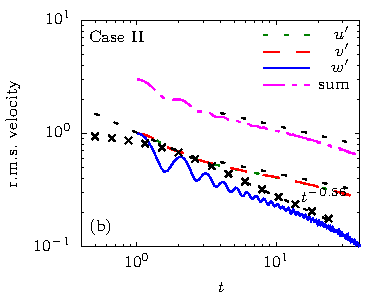
\includegraphics{urmsR600F2}
 \includegraphics{urmsR2325F2}
 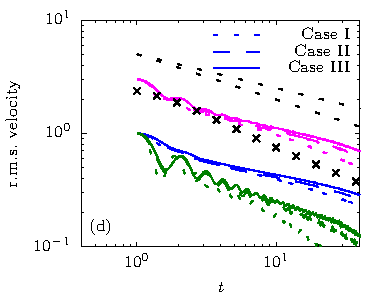
\includegraphics{urms}
\end{center}
 \caption{R.m.s\ velocities versus time $t$. Symbols are for non-stratified cases
   (only for Case I in panel (d)).  The reference slopes are determined by
   least-squares fits to the logarithms of the data in the adjacent lines or
   symbols. 
   %({\bf Need more explanation here?} {\it Isn't it clear from the plots that the dashed lines are ever so slightly offset from, and have the same slope as, one of the coloured lines?}) 
%   \citet{davidson10}.
\label{fig:urms}
}
\end{figure}
%%
\begin{figure}
\begin{center}
  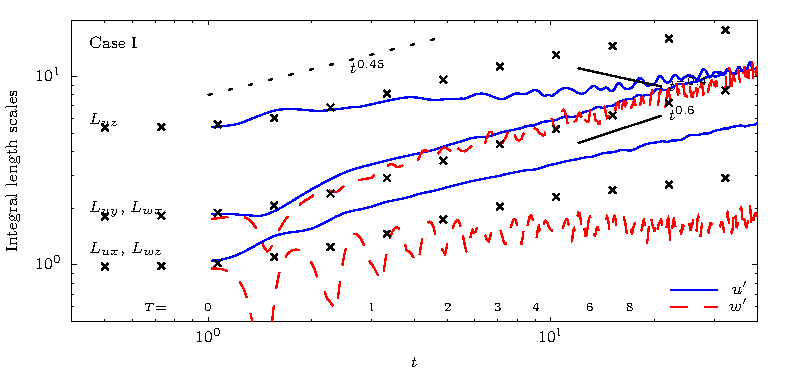
\includegraphics{allLengthsR160F2}
    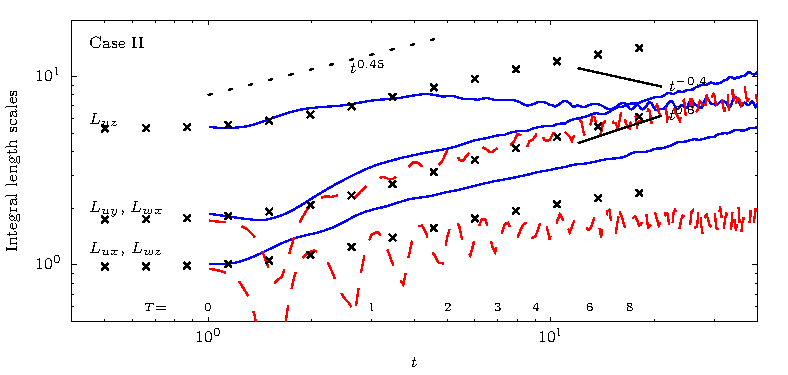
\includegraphics{allLengthsR600F2}
 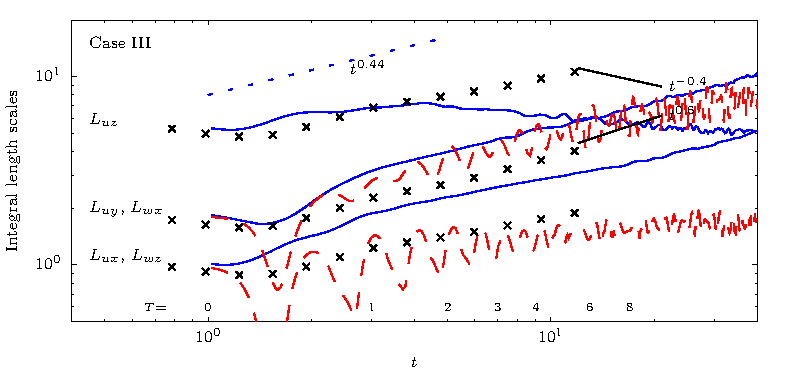
\includegraphics{allLengthsR2325F2}  
\end{center}
 \caption{Integral lengths versus $t$.  The longitudinal scales are plotted true and the
   others are offset vertically in increments of half decades.  The symbols are for non-stratified cases.  The
   dashed-line reference slopes are $1-n$ from the non-stratified simulations.
   The solid-line reference slopes are as derived in \citet{davidson10}.
 \label{fig:intls}}
\end{figure}
%%
In the figure, the symbols representing the non-stratified flow data lie on
curves corresponding to $n=0.56$, 0.56, and 0.55 for Reynolds numbers 160 (Case I),
600 (Case II), and 2325 (Case III), respectively.  These are consistent with the expectation that
$n\approx 0.6$.
%Finally, recall
%that the fields are forced to be stationary, then allowed to decay, and then the stratification is applied %at $t=1$.

%%
%%
%\subsubsection{Time scales}
%
%Having established the virtual origin and decay exponent for the
%non-stratified cases, we consider the stratified cases.  Recall that the
%origin for time $t$ has been taken to be the virtual origin defined in the
%non-stratified flow simulations, and that the density stratification is applied
%at $t = 1$.  There are two time scales of interest in decaying stratified
%flows.  One is the advective time scale, which in dimensional terms is $\hat
%t_{{LE}} = \hat L/\hat U$.  The second time scale is the buoyancy period,
%which in dimensional terms is $\hat T_{{B}} = 2 \pi/\hat N$.  It is usual to
%examine the flow variables as functions of $t$, i.e., time scaled by the
%advective time $\hat t_{LE}$. It is sometimes useful, however, to observe the
%flows in terms of the number of buoyancy periods after stratification has been
%applied, that is, in terms of $T$ defined by
%%
%\begin{equation*}
%T = \left(\hat{t} -\hat{t}_0
%-\frac{\hat{L}}{\hat{U}}\right)\biggl /\hat T_{{B}} = \frac{t - 1}{\F} \ .
%\end{equation*}
%%
%Both times will be used in presenting our results.
%\citet{spedding96b} note that, in laboratory experiments of wakes, it is not possible to align the origins of the turbulence and buoyancy time scales.  In
%the current simulations, however, we were able to very nearly align the origins
%so that $t=1$ is the time at which the buoyancy force is applied and almost
%the time that power law decay is observed in the figures.  For $\R=2325$ for
%instance, the symbols representing the simulation results coincide with the
%line for power-law decay by about $t=0.1$.  Alignment of the time scales is
%not required, but it is convenient when considering plots on logarithmical
%axes.

%%
%%
\subsubsection{Power-law scaling in the stratified flows}
%
Also plotted in figure \ref{fig:urms} are the r.m.s.\ velocities and in
figure~\ref{fig:intls} the integral length scales for the three stratified
cases, the latter which are computed as recommended in Appendix~E of \cite{comte71}.
The notation $L_{ux}$ denotes the integral length scale of
$u$ in the $x$-direction, and similarly for the other length scales.

Consider first the r.m.s.\ velocities, which are plotted in
figure~\ref{fig:urms}.  There is an adjustment immediately following the onset
of stratification at $t=1$, the abruptness of which can be observed in the
evolution of the r.m.s.\ density in figure \ref{fig:rho}.  By about $t=3$
($T=1$, {\em i.e.}, one buoyancy period), the decay rates for $u'$ and $v'$
begin to deviate from their non-stratified values, and settle into power-law
decay rates which are less than the non-stratified values.  Furthermore, from
figure~\ref{fig:urms}d, it is seen that the decay rates are very weakly
dependent on the Reynolds number, with the lowest decay rate observed for Case
III, the case with the highest Reynolds number.  This observed decrease in the
decay rate due to stable stratification is consistent with the prediction of
\cite{davidson10}, although the decay rates are slightly less (in absolute
value) than his estimate of $t^{-0.4}$.  The reduction in decay rate is also
qualitatively consistent with the experiments of \cite{lin79},
\cite{spedding97}, \cite{yoon90} and \cite{stillinger83}, and with the
observations of \citet{almalkie12a} who, in simulations forced to maintain
constant energy in a narrow band of small wave numbers, observed that stronger
stratification slightly reduces the dissipation rate.  These results are
inconsistent with the laboratory experiments of \cite{liu95}, however, who
finds a decay rate of the horizontal velocities of about $n=0.825$ with
stratification, {\em faster} than the rate of 0.65 for his non-stratified
case.  It is also inconsistent with the results of \cite{praud05} who found
the decay rate of about $n=0.65$ for all their nonstratified and stratified
cases.  Note that, in our simulations with stable stratification, after some
initial adjustment, $w'$ decays at almost the same rate as with no
stratification for cases II and III.  When the Reynolds number is low (Case I
at later times) though, $w'$ decays faster with stratification than without.
This is most easily observed in figure\ \ref{fig:urms}d.
%It may be that the dynamics in the flows of \citet{liu95} and \citet{praud05} have some characeristics similar to those of Case I at later times.  (THIS NEEDS SOME EXPLANATION.)

%%
\begin{figure}
\begin{center}
  \includegraphics{rho}
\end{center}
 \caption{R.m.s.\ of the fluctuating density $\rho'$ versus time $t$.  The
   dashed reference slopes are from the total r.m.s.\ velocities in the
   stratified cases.  The solid reference slope is for the r.m.s.\ velocity in
   the unstratified case I.
 \label{fig:rho}}
\end{figure}

In figure~\ref{fig:intls} it is seen that the growth rates of all the
horizontal integral length scales are enhanced by the density stratification.
The growths of the vertical integral scales of $u'$, however, are so
strongly affected by the stratification as to become negative at later times
for cases Case II and Case III.  Both of these results are qualitatively
consistent with the predictions of \cite{davidson10}.  The result for the
vertical scales is consistent with the suggestion by \cite{lilly83} that, as
the effects of stratification become important, the vertical shearing of the
horizontal velocities increases.  It is also consistent with the scaling
analysis of \cite{bil01}.  The fact that all but the vertical lengths are
larger in the stratified cases than in the non-stratified cases does not
necessarily mean that coherent structures are larger, but rather that the
small scales are suppressed.  This will become more apparent when we discuss
energy spectra.  Note that the strong oscillations in the integral length
scales for the vertical velocities are caused by the oscillatory exchanges of
kinetic and potential energies, as the flows respond to the stable
stratification.  This is seen in the oscillations in $w'$ in figure~\ref{fig:urms}, and will become more clear when plots of the time dependence of the potential energy and the buoyancy flux are examined in figures~\ref{fig:rho} and \ref{fig:buoyancyFlux}.  Also note that, when these oscillations are averaged out, the
growth rates of $L_{wz}$ are almost the same as for the non-stratified case.
%{\bf this should be better understood after seeing the curves for potential
%  energy.}

The r.m.s\ of the density fluctuations provides yet another measure of the
decay rate of stratified turbulence.  For a passive scalar $\phi$ in isotropic
turbulence with $u' \propto t^{-n}$, similarity analysis and data indicate
that $\phi' \propto t^{-n}$ as well \citep[c.f.][]{debk00a}.  Since the stratified
flows exhibit different decay rates for the horizontal and vertical
velocities, we might not expect the decay rate of the scalar fluctuations to
agree with that of any single velocity component.  From figure
\ref{fig:rho}, however, it is observed that for cases II and III the decay rate of the density fluctuations is almost the same as that of the total r.m.s.\ velocity.  Interpreting $\rho'^2$ in terms of potential energy (see \S\ref{flow-energetics}), this implies that the potential energy decays at almost the same rate as the horizontal components of the kinetic energy for these cases.  Significant Reynolds number effects are observed in the figure.  For
the case with lowest Reynolds number, the decay rate of the scalar
after $T=1$ is faster than for the total r.m.s.\ velocity.  At later times in
this case (Case I), the decay rate is even faster than for the non-stratified
simulation, consistent with it following decay rate of $w'$.  Recall
that \citet{liu95} and \citet{praud05} observed that stratification increased
the decay rate of velocity, especially the vertical velocity, and so our Case I at later times may provide some
insight into the dynamics of those laboratory experiments.  This issue will be addressed further in \ref{late-time}

%%
%%
\subsubsection{Froude number dependence}
%
\begin{figure}
\begin{center}
 \includegraphics{froude}
% \includegraphics[width=5in]{reynolds}
\end{center}
\caption{Horizontal Froude number $\Fh$ versus time $t$.}
%\end{center}
\label{fig:froude}
\end{figure}

The temporal decay of the horizontal Froude number, defined as $\Fh = 2 \pi
\hat u_h/\hat L_{ux} \hat N$, is seen in figure~\ref{fig:froude} for all three
cases.  Here $\hat u_h$ is the dimensional r.m.s.\ horizontal velocity and
$\hat L_{ux}$ is the dimensional analogue of $L_{ux}$.  The decay curves are
very similar for all three different Reynolds numbers, although at late time
Case I is decaying slightly faster.  Furthermore, as
suggested by \cite{riley81}, $\Fh < {\cal O}(1)$ for about $T > 1$,
indicating that stratification begins to dominate in this temporal region.  This is
consistent with the results in figures~\ref{fig:urms} and \ref{fig:intls},
where the velocity decay rates and integral scale growth rates change somewhat
abruptly near $T = 1$, as the flows enter the strongly stratified regime.

%%
%%
\subsubsection{Flow energetics}
\label{flow-energetics}
%
Information regarding the energy decay rates is given in figure \ref{fig:energy}.  
%({\bf Is something wrong with this figure?  Since $u_h'$ and $\rho'$ decay at %approximately the same rate, then shouldn't $E_h$ and $E_p$?})  
Here $E_h$ is the kinetic energy associated with $u$ and $v$,  and $E_v$ is that associated with $w$.  We define $E_p$, the potential energy of the density fluctuations relative to the ambient density, as
\begin{equation*}
E_p = \frac{1}{2} \biggl ( {\frac{2 \pi}{Fr}} \biggr )^2 \rho'{^2}. 
\end{equation*}
$E_p$ can be considered as a surrogate for available potential energy
\citep{lorenz55}.  
%and $E_p$ is the potential energy associated with the density fluctuations relative to the ambient
%density and so is a surrogate for the available potential energy.  
In panel (a) of the figure, all the energies have been normalised by the local
(in time) total energy, i.e., by $E_h+E_v+E_p$.  From this panel it is
observed that the horizontal components of the kinetic energy become
increasingly dominant over the sum of the vertical component and the potential
energy.  This could be due to one or more of several effects.  Possibly
internal waves are being absorbed by the more horizontal motions, as in the
laboratory experiments of \cite{godoy-diana06}, leading to a decrease in both
$E_v$ and $E_p$ while enhancing $E_h$.  Furthermore, as kinetic energy is
exchanged with potential energy through the action of the buoyancy flux
$-(2\pi/\F)^2 \left<\rho w\right>$, with $\left< \cdot \right>$ denoting a
spatial average over the entire domain, the dissipation rate of potential
energy $\chi$ (see section \ref{dissipation rates}) provides another avenue
for dissipation in addition to the kinetic energy dissipation rate $\epsilon$.
From this panel, it is also observed that the partition between the
contributions to total energy depends on the Reynolds number, since Reynolds
number is the only parameter that is varied between the simulations.
%Unfortunately \citet{praud05},
%hereafter abbreviated PFS, due to experimental limitations, are not able to identify either the change in decay rate
%due to stratification nor the Reynolds number dependence, but the laboratory
%data are not as clean as that from the DNS and so precise comparisons are not
%possible.  Power-law decay of kinetic energy is shown in figure
%\ref{fig:energy}(b), including a reference line with the exponent -1.3
%reported for the PFS data.  It is evident that laboratory flows decay faster
%than the simulated ones.  Also, it is reported for the PFS data that vertical
%motion accounts for less than 1\% of the kinetic energy over the range of time
%that the decay exponent is measured whereas it is not this low in the DNS.  It
%may be that since the simulated flows are given time to develop before
%stratification is imposed that the effective initial Reynolds number in the
%simulations is significantly higher than in the PFS data.  
This Reynolds number dependence is not surprising.  For example,
\citet{perot06} reported, from examining many sources, that the decay
exponents for non-stratified turbulence are larger in magnitude for lower
Reynolds numbers.  Finally, note from panel~(b), and the fact that the
non-stratified energy decay rate is approximately $t^{-1.1}$, that the decay
rate of the total energy is inhibited by the stratification, consistent with
the inhibition of the decay rates of the horizontal components of the velocity.
%it may be that
%a DNS with Reynolds number lower than that in R160F2 might more closely match
%the PFS data both in the decay exponent for energy and the fraction of kinetic
%energy due to vertical motions.

\begin{figure}
\begin{center}
 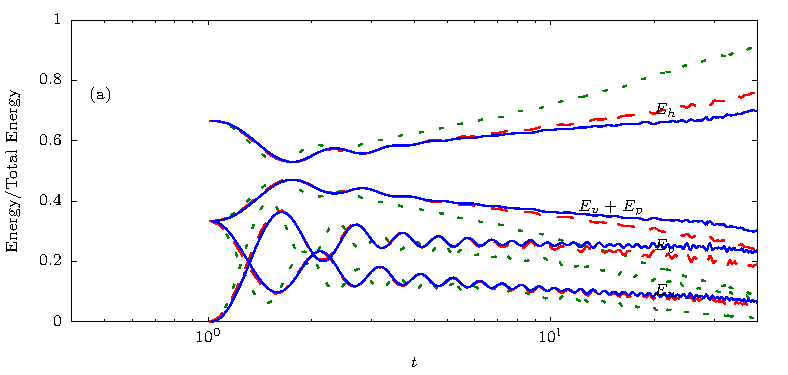
\includegraphics{keRatio}
 \includegraphics{te}
\end{center}
 \caption{(a) Ratio of energy contributions to total energy versus
   time.  (b) Total energy versus time.  In places where it is
   difficult to see the curves for Case II, they almost coincide with those for
   Case III. In panel (b), the two reference slopes correspond to $n=-0.55$ and $n=-0.28$ on figure \ref{fig:urms}c.  
%   ({\bf It is difficult to distinguish the reference slopes from the other curves in %(b).})
\label{fig:energy}}
\end{figure}

The behaviour of the buoyancy flux for all three stratified cases is seen in
figure~\ref{fig:buoyancyFlux}.  The oscillations about 0 in the buoyancy flux in figure~\ref{fig:buoyancyFlux}(a)
represent net exchanges from the vertical component of the kinetic energy to
potential energy (positive values) and back from potential into kinetic energy
(negative values), consistent with the plots of these components of the
energy.  The period of oscillation is about $0.4 T_B$ for the case Case~I, and
appears to lengthen slightly with Reynolds number.  These oscillatory results
are qualitatively consistent with the numerical simulations of \cite{riley81} and the laboratory 
experiments of \cite{liu95}.  Figure~\ref{fig:buoyancyFlux}(b) is a plot of the cumulative (integrated) value of the buoyancy flux, divided by the initial total energy, giving the net transfer of kinetic into potential energy.  It is seen that, for cases II and III, the cumulative flux asymptotes to approximately 30\% of the initial total energy.  Also note that the cumulative flux is somewhat smaller for Case I, the lowest Reynolds number case.  These facts are closely related to the behaviour of the mixing efficiency $\eta$ discussed in the next section.  
%({\bf It might be interesting to plot the integral of each of these terms versus time to %see if there is a continual net transfer of kinetic to potential or vice-versa.})
%%
\begin{figure}
\begin{center}
 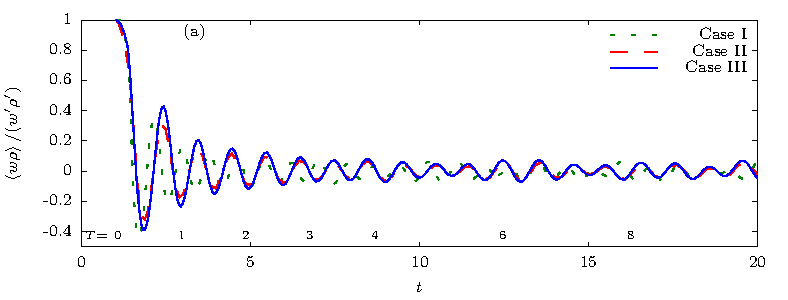
\includegraphics{b}
 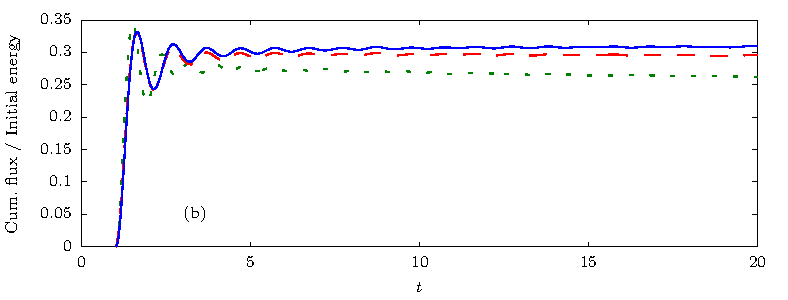
\includegraphics{cum-b}
\end{center}
 \caption{(a) Buoyancy flux, normalised by $w' \rho'$, versus time for all three stratified cases. (b) Cumulative buoyancy flux normalised by initial total energy.
\label{fig:buoyancyFlux}}
\end{figure}


%
%\subsection{Buoyancy flux and potential energy dissipation rate}

%%
%%
\subsubsection{Dissipation rates and mixing efficiency}
\label{dissipation rates}
%
The dissipation rates of potential and kinetic energies are 
$$\chi = \left< \frac{2 \pi} {Fr^2 Pr Re} 
\nabla \rho \cdot \nabla \rho 
\right>
$$ 
and
$$\epsilon = \left< \frac{1}{Re} \boldsymbol{S} : \boldsymbol{S}\right> ,$$
respectively, where $\boldsymbol{S}$ is the non-dimensional strain rate
tensor.
%({\bf We don't define $\epsilon$ with an equation.  I don't think we need to define $\chi$ either.  Just say it is the dissipation rate of available potential energy relative to the time-invariant ambient density.}  
The time evolutions of their averages are shown in
figure~\ref{fig:dissipation}.  Noticeable is the decrease in $\epsilon$ due to
the stratification.  Furthermore, there is a slight decrease and then increase
in $\epsilon$ as the Reynolds number is increased, whereas
there is a slight increase in $\chi$ as it is increased.  Also
evident is that the non-stratified cases are not quite in power law decay at
$t=1$, which is also apparent in figure \ref{fig:urms} for all the
non-stratified cases; however power law decay does occur in the non-stratified
simulations well before $T=1$.  In addition note that, after the flow
adjustment, the ratio of $\chi$ to $\epsilon$
is about 0.54 except for the lowest Reynolds number case, where the ratio
continues to decrease in time.  We will find below in \S\ref{late-time} that,
for this lowest Reynolds number case (Case I), the flow might not be fully
turbulent beyond about 2 buoyancy periods.

\begin{figure}
\begin{center}
 \includegraphics{chi}
\end{center}
 \caption{$\epsilon$ (upper curves), $\chi$ (lower curves).  Symbols are for
   Case III with no stratification.
\label{fig:dissipation}}  
\end{figure}

Of special interest is the ratio $\eta \equiv \chi/(\chi + \epsilon)$, which
is sometimes taken to be the definition of the mixing efficiency
\citep{osborn80,smyth01}.  From figure~\ref{fig:mixing_efficiency} it is seen
that, for the higher Reynolds number cases, $\eta$ asymptotes to a value of
about 0.35, compared to the value of 0.3 obtained by \cite{riley03} in a
similar regime, to 0.25 obtained by \cite{maffioli16b} at very low Froude
number, to 0.41 inferred from the data of \cite{liu95}, and 0.17 assumed by
\cite{osborn80} based upon ocean data.  In the forced homogeneous simulations
reported by \citet{debk16a}, $\eta$ ranges from 0.22 at $\Fh=0.22$ (computed
in the same way as it is for the current simulations), to 0.37 at $\Fh=2.8$.
Note that the value for $\eta$ of 0.35 is consistent with the asymptotic ratio
of $\chi/\epsilon$ of about 0.54, as found in figure~\ref{fig:dissipation}.

\begin{figure}
\begin{center}
 \includegraphics[width=5in]{eta}
 \end{center}
\caption{Mixing efficiency $\eta= \chi/(\chi + \epsilon)$}
%\end{center}
\label{fig:mixing_efficiency}
\end{figure}

There is some evidence that $\eta$ depends on the Prandlt (or Schmidt) number.
For example, from numerical simulations of stratified shear flows, \cite{smyth01} found that $\eta$
decreased from 0.35 to 0.22 as the Prandlt number increased from 1 to 7.  More
recently \cite{salehipour15} found in numerical simulations of stratified
shear flows that $\eta$ decreased from 0.24 to 0.18 as the Prandlt number
increased from 1 to 16.  \cite{salehipour15} also gave some physical and
mathematical reasoning for this decrease with Prandlt number.  For a subset of the simulations of \citet{debk16a} run with $Pr = 7$, $\eta$ ranges from 0.17 at $\Fh = 0.4$ to 0.28 at $\Fh = 2.8$. 
%{\bf We should
%  check these numbers.  Steve, should we add some comments on your recent
%  simulations here?}

%%
%%
\subsubsection{The buoyancy Reynolds number and activity parameter}
\label{activity}
%
Dimensional reasoning suggests that three initial parameters are required to describe
decaying, homogeneous, stratified turbulence.  For
equations~\eqref{eq:governing}, these are chosen to be the Prandtl number,
$Pr$, in addition to the Reynolds and Froude numbers, $Re$ and $Fr$.  The
latter are defined here in terms of the integral length scale $\hat{L}$ and
r.m.s.\ velocity $\hat{U}$ of the simulated flow at $t=1$, {\em i.e.}, before
there is any effect of stratification. The conditions at $t=1$ provide a
useful basis for non-dimensionalising the flow statistics.  To better understand the effects of stable stratification, however, it is useful to consider the local in time values of $Re$ and $Fr$.  Because of the non-isotropy which develops in the flows, the corresponding vertical and horizontal scales in the flow differ significantly, as seen in figure~\ref{fig:intls}.  Therefore, considering the local r.m.s.\ horizontal velocity $u_h$, one can define two Froude numbers of potential importance, $\Fh = u_h/N L_{ux}$ and $\Fv = u_h/N L_{uz}$ based upon the horizontal longitudinal integral scale $L_{ux}$ and the vertical lateral integral scale $L_{uz}$, respectively.  From the scaling arguments of \cite{bil01}, at least for large $\R$, it is found that $\Fv$ should remain ${\cal O}(1)$, so that its local in time behaviour need not be considered.  Therefore, it is important to locally consider only $\Rh$ and $\Fh$, where $\Rh$ is also based upon $u_h$ and $L_{ux}$.  As reviewed in \S\ref{sec:introduction},
these two parameters combine to form $\Rb = \Fh^2 \Rh$, whose potential
relevance is based on the shearing dynamics observed to occur when strong
stratification leads to the tendency for vertical decoupling of horizontal
motions \citep{riley03}.

In the stratified turbulence literature, $\Rb$ is often referred to as the
`buoyancy Reynolds number,' a terminology we have adopted in this paper.  In the
geophysical literature, this terminology usually denotes
%%
\begin{equation}
\Gn \equiv \frac{\hat{\epsilon}}{\hat{\nu} \hat{N^2}} = \Ft^2 \Rt \ .
\end{equation}
%%
Here the turbulence Froude and Reynolds numbers, $\Ft$ and $\Rt$, are defined
in terms of the turbulence length scale $\hat{\ell}=\hat{U}^3 /
\hat{\epsilon}$, with $\hat{U}$ being the total r.m.s.\ velocity.  These are
the definitions used in \citet[e.g.][]{brethouwer07}; however, they refer to
$Gn$ as the buoyancy Reynolds number.  (Note then that $\Rb$ and $Gn$ differ in the
choice of their characteristic velocity and characteristic length scales.)  We
use the symbol $\Gn$ in deference to the introduction of this quantity by
\citet{gibson80}, and to its identification by \citet{gargett84} as a measure
of the scale separation available for turbulence between the Ozmidov, $\hat
L_o = (\hat \epsilon/\hat N^3)^{1/2}$, and Kolmogorov, $\hat L_k = (\nu^3/\hat
\epsilon)^{1/4}$, length scales; we call $Gn$ the `activity parameter'
following some of the early literature on the subject
\citep[e.g.][]{dillon84}.  

In figure~\ref{fig:gn} the evolution of $\Rb$ and $Gn$ in time are shown. 
%while
%the trajectories of simulation cases I, II, and III through the $\Fh$-$Gn$
%plane are given in figure~\ref{fig:gn}(b).  
Note that, as seen in terms of their decay rates in figure~\ref{fig:gn}, $\Rb$ and $Gn$ are not proportional in the present
simulations, so that they cannot be used interchangeably.  Also note that there is a change in slope in $\Rb$ at about $T=1$, consistent with the results for $u$ and $v$ seen in figure~\ref{fig:urms}. It is also apparent that $\Rb$ scaled by the initial Reynolds number
evolves differently for Case I than for Cases II and III.  All three cases evolve in a similar manner up to about $T=2$, at which point Cases II and III
appear to diverge from Case I.
%This observation includes some subjectivity, but consider it in the context of
%the bottom figure in the panel by following each curve from right to left.
%For Case I, there is a single change of slope at about $T=1$.  For the Case II
%there are two changes of slope, one at about $T=1$ and the second at about
%$T=2$.  For case II there are also two changes of slope, one at about $T=1$
%and the second at about $T=4$.  

Our hypothesis is that the differences in the evolution of the three cases,
evident in figure~\ref{fig:gn}, can be explained by when $Gn$
drops below $O(1)$, as will be discussed more in \S\ref{late-time} on late time results.  \citet{gibson80} predicted that $Gn > 30$ is necessary
for sustained turbulence, a value supported experimentally by
\citet{stillinger83}.  In simulations of forced homogeneous stratified
turbulence with $Gn=13, 48,$ and 220 \citep{portwood16}, only in the case with
$Gn=220$ is there a range of length scales in which the turbulence is
approximately isotropic throughout much of the simulation domain, although all
the cases exhibit at least some patches of approximately isotropic turbulence.
Even in the case with $Gn=220$ there is no range of scales consistent with the
assumptions of Kolmogorov, Oboukhov, and Corrsin regarding inertial and
convective subranges
\citep{kolmogorov41,oboukhov41a,oboukhov41b,oboukhov49,corrsin51,kolmogorov62,oboukhov62}.
For the same three data sets, \citet{portwood16} find that at $Gn=220$ the
domain is dominated by space-filling patches of turbulence, while when $Gn=13$
and 48 the simulated flows consist of a mixture of space-filling patches and
horizontally-layered turbulence.  As seen in figures~\ref{fig:rhocontours} and \ref{fig:gnslice}, the flows studied here become very layered beyond about $T=2$.

%Recall that the potential relevance of $\Rb$ as a
%parameter to describe stratified turbulence is based on the flow consisting of
%layered turbulence ({\bf but $Gn$ is being discussed?}).

%%
\begin{figure}
\begin{center}
 \includegraphics{reynolds}
%  \includegraphics{Fh-Gn}
\end{center}
 \caption{$\Rb$ and $Gn$, normalised by the initial Reynolds number, versus $t$.
}
 \label{fig:gn}
\end{figure}
%%

Turning now to $\Rb$, \citet{riley03} have argued that shear instabilities can
be expected to occur in the strongly stratified regime provided $\Rb > O(1)$.
This criterion has been verified, to some extent, by the simulations of
\cite{deloncle08} and refined by \cite{augier11}.  It is seen that, for all
the cases and all the times, $\Rb/Re$ is greater than about 0.1, and so that,
approximately, $\Rb > 15$, indicating that that we would expect shear
instabilities to continue to exist for these flows.  These instabilities would
only be expected to lead to turbulence, however, when approximately $\Gn >
0.5$.


\citet{hebert06b} present data from 14 simulations of decaying stratified
turbulence that indicate $\Rb \propto Gn$, but each simulation is sampled at a
single time, not as a function of time.  For the current simulations, the plots of $\Rb$
and $Gn$ versus time in figure \ref{fig:gn} indicate that $Gn$ decays more rapidly than does $\Rb$ for all three cases; therefore there is no
proportionality between $Gn$ and $\Rb$ and, in all three cases, the ratio $\Rb/Gn$ increases with
time. 
%({\bf Should this ratio be plotted?})
The ratio of $Gn$ to $\Rb$ is closely related to the ratio of the integral to the turbulence
length scales, $L_h$ and $\ell = u_{rms}^3/\epsilon$, {\em i.e.,} the ratio
%%
\begin{equation}
{\mathcal D} \equiv \epsilon L_h / u^3_{rms} \, .
\end{equation}
%%
To be precise, $Gn/\Rb$ includes a factor of the ratio of the
r.m.s.\ horizontal velocity to the r.m.s.\ total velocity, and there is an
additional factor of $2\pi^2$.  ${\mathcal D}$, however, is well known in the
study of nonstratified turbulence and so we turn our attention to it rather
than $Gn/\Rb$.  \citet{pope00} shows that, when the ratio is computed from a
model spectrum, it depends on the Reynolds number over the range of Reynolds
numbers accessed by all but a few numerical simulations and laboratory
experiments in homogeneous, isotropic turbulence.  From an examination of
results from a number of laboratory experiments and numerical simulations,
\citet{sreenivasan98} reports ${\mathcal D}$ in the range of about 0.4 to
1.81.
%which is the basis for the
%grey band in figure \ref{fig:gn} ({\bf We need to explain the grey band better.}).  %Sreenivasan 
He also notes that simulations of
homogeneous, isotropic turbulence by multiple researchers can be divided into
two groups, with ${\mathcal D}$ for one group of simulations being consistent
with each other but markedly higher than for the other group, for which
$\mathcal D$ is consistent with the analysis of Pope.  For decaying
homogeneous stratified simulations, \citet{maffioli16} report ${\mathcal D}$
as low as 0.3.  \citet{hebert06b} report ${\mathcal D} \approx 0.4$ for their
snapshots of the 14 decaying cases referenced above. For the simulations of
forced stratified turbulence with $Gn=13$, 48, and 220, \citet{debk15} reports
${\mathcal D} =0.53$ at $Gn=220$ and 0.57 at $Gn=13$.  Sreenivasan reports
that ${\mathcal D}$ tends to be higher for forced cases.  We note that
typically in forced simulations, and certainly in those of \citet{debk15}, the
large scales are not as well resolved as in decaying simulations, which adds
to the difficulty in accurately estimating $L_h$.

Data for $\mathcal D$ for the current simulations are shown in figure
\ref{fig:RR/Rb}.   
%%
\begin{figure}
\begin{center}
 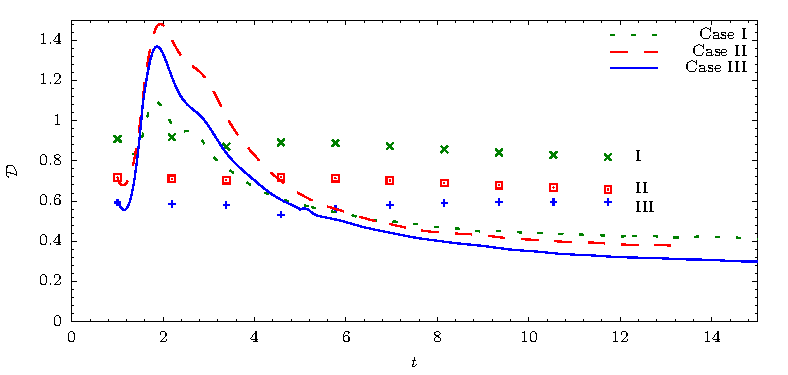
\includegraphics{D1}
%    \includegraphics{R_vs_Reb}
\end{center}
 \caption{Length scale ratio.  
 \label{fig:RR/Rb}}
\end{figure}
%%
For the non-stratified cases, the values are consistent with those collected by
\citet{sreenivasan98}, and they exhibit the expected trend of increasing with
decreasing
%Taylor 
Reynolds number from one simulation to the next.  
%({\bf should we give the Taylor Reynolds numbers?})  
The results for the 
stratified cases go through an adjustment period at early time and then trend
toward the range 0.3 to 0.4, consistent with the decaying cases of
\citet{hebert06b} and \citet{maffioli16}.  The lower values of ${\mathcal D}$
for the stratified cases are consistent with the decrease in $\epsilon$ and the
increase in both $u_{h}$ and $L_h$.
%\afterpage{\clearpage}

%%
%%
\subsubsection{Energy spectra}
%%
\begin{figure}
\begin{center}
\includegraphics{compensated}
\end{center}
\caption{Uncompensated (a) and compensated (b) longitudinal spectra of $u$ averaged with that of $v$.}
 \label{fig:h-spec}
\end{figure}
%%
%%
%%
%\begin{figure}
%\begin{center}
%\includegraphics{R2325v}
%\end{center}
%\caption{Vertical spectra of all velocity components (a) and of $u$ (b).  In panel (a), %the spectra are offset in the vertical for clarity.  }
% \label{fig:v-spec}
%\end{figure}
%%
%%


%\cite{riley03} found that, for decaying, strongly stratified turbulence at a
%high enough Reynolds number, the horizontal spectra of the horizontal
%velocities exhibited an approximate -5/3 behaviour in the spectral range
%roughly between the energy peak and the Ozmidov scale.  Later
%\cite{lindborg06a} gave a theoretical rationale for this behaviour, arguing
%that, if the horizontal Froude number is small enough so that there is some
%scale separation between the energy-containing range and the Ozmidov scale,
%the spectra should depend only on the spectral transfer rate, $\epsilon$, and
%the horizontal wave number, leading to the -5/3 result.  He also supported his
%argument with some results from numerical simulations and some data from field
%experiments; several other authors find similar spectral behaviour in numerical
%simulations (e.g., \cite{brethouwer07}, \cite{maffioli16}).  
%More recently -5/3 spectral behaviour has been found in horizontal spectra, but
%not vertical spectra, in a river near its river surface under calm conditions
%\citep{chickadel11} and in numerical simulations \citep{flores17} under
%similar conditions. The river surface under calm conditions can of course be
%considered a strongly stratified layer.

%To satisfy Lindborg's assumptions, it is required that a flow be at very low Froude
%number, but very high Reynolds number, necessitating sufficient separation
%between the Kolmogorov, Ozmidov, and energy-containing scales.  Because scale separation %is limited in simulations, \citet{debk15} found that it is important to consider %compensated spectra so as not to confuse the top of the dissipation range with the %inertial range.  

The horizontal velocity spectra $E_{xx}$ versus horizontal wave number $\kappa_x$ are plotted in figure~\ref{fig:h-spec}(a), where the spectra of $u$ has been averaged with that of $v$. The corresponding compensated horizontal spectra versus horizontal wave number times the Kolmogorov length scale $L_k$ are plotted in figure~\ref{fig:h-spec}(b).  It is seen that, at $T = 0.0$, when the stratification is applied, the non-stratified spectrum has a moderate inertial range.  The compensated spectrum in figure~\ref{fig:h-spec}(b) is consistent with the Kolmogorov constant of about $C_1=0.53$, which is slightly higher than the value of $0.49$ in \citet{pope00} but well within the range for the many data sets reviewed by \citet{sreenivasan95}. 

In isotropic turbulence at high enough Reynolds numbers, there is found a bump in the compensated spectrum to the right of $\kappa L_k \approx 0.02$, which is sometimes attributed to a "bottleneck" of energy transferring to smaller scales. \citet{meyers08} review efforts to understand and model this phenomenon.  \citet{debk15} shows that stratification suppresses this bump and that the -5/3 slope can occur at the top of the dissipation range even though it does not occur in the inertial range.  The suppression of the bump by stratification is consistent with the hypothesis that the bump is due to the bottlenecking of the energy transfer rate combined with the observation that, for the current simulations, stratification reduces the energy decay rate, and hence the energy transfer rate.

Note that in figure~\ref{fig:h-spec}(b) there is a bottleneck bump to the right of $\kappa L_k \approx 0.02$ at $T=0$.  By $T=0.5$ the bump has been suppressed and a peak in the spectrum has begun to develop in the range where the inertial-range plateau exists at $T=0$.  By $T=1.2$, the spectrum is very similar to those in figure 4(a) of \citet{debk15}.  This is somewhat surprising because it has been assumed that the peak in the spectra is an artefact of the energy forcing used to maintain the statistical stationarity of those simulations, yet in the current simulations there is no forcing.  The plots of the compensated horizontal spectra are also qualitatively similar to those obtained by \cite{maffioli16}, and in fact the growth of the spectra in the low wave number region, and the decay in the high wave number region, are also consistent.

% Note that the scale separation between the energy-containing scale and the Ozmidov scale can be seen by computing the ratio $\hat L_o/\hat L_{ux}$, i.e., in terms of non-dimensional quantities,
% \begin{equation*}
% {{\hat L_o} \over {\hat L_{ux}}} = \biggl ( {{\hat \epsilon} \over {\hat \nu \hat N}} \biggr )^{1/2} = \biggl ( {{\epsilon \hat U^3} \over {\hat L \hat N}} \biggr )^{1/2} {1 \over {L_{ux} \hat L}} = {\epsilon^{1/2} \over L_{ux}} Fr^{3/2} \, . 
% \end{equation*}
% At $T = 3$, $\epsilon \approx 1.5\cdot10^{-2}$ (see figure~\ref{fig:dissipation}) and $L_{ux} \approx 2.5$ (see figure~\ref{fig:intls}), so that, with $Fr = 2$, the $\hat L_o/\hat L_{ux} \approx 0.13$.  So the scale separation between $\hat L_{o}$ and $\hat L_{ux}$ is a little less than one decade, which is consistent with the breadth of the approximate -5/3 region in the figure.  {\bf should we instead bring in the buoyancy Reynolds number?}

%%
\begin{figure}
\begin{center}
  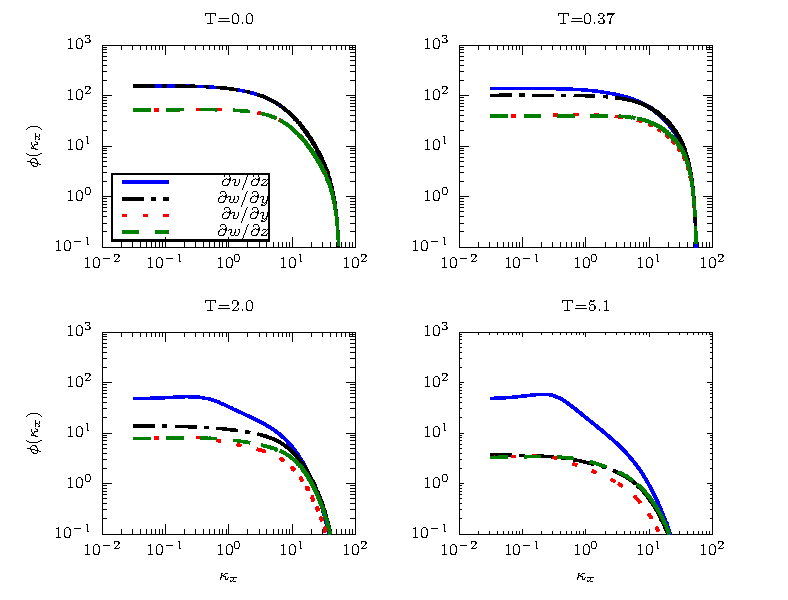
\includegraphics{issf_shear}
\end{center}
\caption{Horizontal spectra of various shear terms.}
 \label{fig:spec-shear}
\end{figure}
%%

The question arises regarding whether a stratified turbulence inertial range, as proposed by \cite{lindborg06a}, should be expected for our simulations.The possibility for this to occur will depend upon (i) the ratio of the energy-containing range scale, characterized by $L_h$, to the Ozmidov scale $L_o$; and (ii) the ratio of the Ozmidov scale to the Kolmogorov scale, given by $Gn^{4/3}$.   A stratified turbulence inertial range would be expected to exist between the energy-containing and Ozmidov wave numbers, so that $L_h/L_o$ should be at least 100 or more.  Furthermore, for turbulent behaviour to exist, we find in \S\ref{late-time} that $Gn$ must be at least of order 1.  Considering the highest Reynolds number case (Case III), we find that at $T=1$, where the flow becomes strongly affected by stratification, $L_h/L_o = 32.3$, while $L_o/L_k = 10.1$.  Clearly the ratio of $L_h/L_k$ is not large enough for an inertial range to exist.  When the ratio of $L_h/L_o$ becomes large enough for the inertial range to exist, at $T=6$, where $L_h/L_o = 216$, then $L_o/L_k$ has dropped to 1.4, which is too small to expect active turbulence.  Therefore we conclude that there is not enough separation of scales for a stratified flow inertial range to occur.  The flow would have to be started at a substantially higher Reynolds number for the possibility to exist.

Some additional insight into the dynamics of strongly stratified flows can be seen from examining the horizontal spectra of various components of the velocity gradient tensor.  Figure~\ref{fig:spec-shear} contains plots of the $k_x$ spectra of $\partial v/\partial z$, $\partial w/\partial y$, $\partial v/\partial y$, and $\partial w/\partial z$ for four points in time for Case III, the highest Reynolds number case.   Note that, for isotropic turbulence, it is expected that the spectra of $\partial v/\partial z$ and $\partial w/\partial y$ will be identical, as will the spectra of $\partial v/\partial y$, and $\partial w/\partial z$.  It is clear that at $T = 0$ this is the case.  As the flow evolves, the spectra of $\partial v/\partial y$, and $\partial w/\partial z$ remain approximately the same, although the spectrum of $\partial v/\partial y$ decreases slightly faster than that of $\partial w/\partial z$ at higher wave numbers.  This supports the scaling arguments of  \cite{bil01} that all three terms in the continuity equation, $\partial u/\partial x$, $\partial v/\partial y$, and $\partial w/\partial z$, should be of the same order.  Somewhat surprisingly, the spectra of $\partial w/\partial y$ and $\partial w/\partial z$ become almost identical at the latest time.  What is noteworthy,  however, is the rapid decrease with time of the spectra for $\partial w/\partial y$, $\partial v/\partial y$, and $\partial w/\partial z$ compared to that for $\partial v/\partial z$, with the spectrum for $\partial v/\partial z$ evolving well above the rest.  Furthermore, the peak in the spectrum of $\partial v/\partial z$ remains into smaller wave numbers. Both of these facts are indications of the development of strong vertical shearing of the horizontal motions as suggested by \cite{lilly83}.

%
%\begin{figure}
%\begin{center}
% \includegraphics{urmsR160F2b}
%  \includegraphics{urmsR600F2b}
%   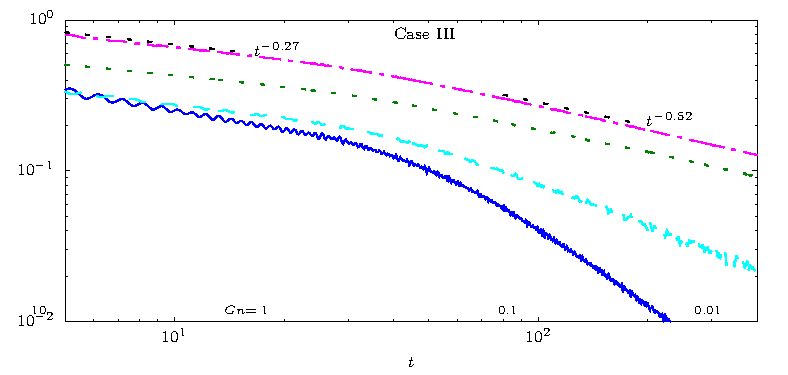
\includegraphics{urmsR2325F2b}
%
%\end{center}
% \caption{Evolution of flows into late time.  
% \label{fig:viscousRegime}}
%\end{figure}
%%
%%
%%
%
%\begin{figure}
%\begin{center}
% \includegraphics{gnslice}
%\end{center}
% \caption{$\log_{10}(\Gn)$ on a vertical slice of Case III %at various times.  Only the upper 1/4 and left 1/2 of the %domain is plotted. \label{fig:gnslice} }
%\end{figure}
%%
%%
%%
%\afterpage{\clearpage}
\subsection{Late time results}
\label{late-time}
%%
%%
We now consider the late time behaviour of these flows, when $\Gn$ falls to ${\cal O}(1)$ and below, and so viscosity becomes a dominating influence. Figure~\ref{fig:viscousRegime} contains plots of $u'$, $w'$ and $E_p^{1/2}$ versus time carried out to 150 buoyancy periods or more for each case, and where $\Gn$ has dropped to values of 0.01 or less at very late times.  Note the $\Gn$ scale at the bottom of each plot, depicting the local values of $\Gn$ at different times for each case.  There are two things to note about these plots. First, for each case, between values of $\Gn$ of 1 and 0.1, $u'$ begins to decay at a slightly steeper rate.  Second, for values of $\Gn$ in this same range, the vertical velocity and $E_p^{1/2}$ (proportional to $\rho'$) begin to decay precipitously, indicating that the flows are becoming quasi-horizontal.  
%%
\begin{figure}
\begin{center}
 \includegraphics{urmsR160F2b}
  \includegraphics{urmsR600F2b}
   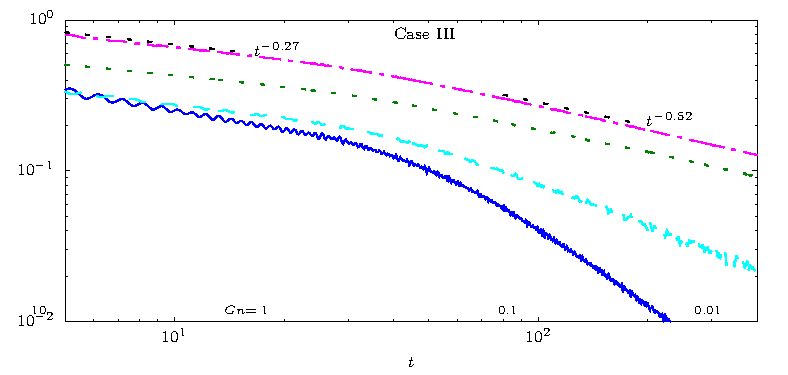
\includegraphics{urmsR2325F2b}

\end{center}
 \caption{Evolution of $u'$, $v'$, $w'$ and $E_p^{1/2}$ into late time.  Reference slopes are shown for $Gn>1$ and $Gn \ll 1$ except for Case I $Gn > 1$ for which is not in the range of times on this figure.  For velocity data at early times see figure \ref{fig:urms}. 
 \label{fig:viscousRegime}}
\end{figure}
%%

These plots can be better understood by examining the trajectory of each flow in the $\Fh$-$\Gn$ plane, as given in figure~\ref{fig:Fh-gn}. Each flow is seen to go through three regimes.  In the first, the flows decay at the non-stratified rate, which is seen in figure~\ref{fig:urms} to occur up to about 1 buoyancy period after flow initiation, when the values of the local Froude numbers have fallen to about 0.6 (see figure~\ref{fig:froude}).  We take this to be the value of $\Fh$ when a flow has entered the strongly stratified regime. The decay rate in this regime diminishes due to the effects of stable stratification, approximately as predicted by \cite{davidson10}.  Finally, in the third regime, when $\Gn$ has decayed to between 1 and 0.1 for each case, the flows become viscously dominated and begin to decay at a faster rate.  Note that this viscous domination had already been observed for Case I at earlier times in the behaviour of $\rho'$ in figure~\ref{fig:rho}, in the behaviour of the various components of energy in figure~\ref{fig:energy}(a), and in the behaviour of the mixing efficiency in figure~\ref{fig:mixing_efficiency}.
%%
\begin{figure}
\begin{center}
%  \includegraphics{reynolds}
  \includegraphics{Fh-Gn}
\end{center}
 \caption{The trajectory of each flow in the $\Fh$-$Gn$ plane.  The symbols mark the time in buoyancy periods, with the corresponding times indicated on the curve for Case~III.
}
 \label{fig:Fh-gn}
\end{figure}
%%

These results are analogous to those obtained in the experiments of \cite{spedding97} discussed in \S\ref{sec:introduction}.  He studied the decay of turbulence in the wake of a towed sphere in a salt-stratified towing tank, and found in measuring the mean axial velocity that, initially, the flow decayed at the non-stratified rate.  But at a time of the order of a buoyancy period, the decay rate decreased appreciably in what he called the non-equilibrium regime.  Further in time, in the region he called the late wake, or quasi-two-dimensional regime, the flow again decayed at a faster rate.  We speculate that in this last regime $\Gn$ had become small in his flows, which would therefore be viscously dominated.  Furthermore the vertical velocity had been suppressed compared to the horizontal velocity, as the flow exhibited a quasi-horizontal vortex structure.
%%
\begin{figure}
\begin{center}
 \includegraphics{froudeLate}
\end{center}
 \caption{Froude numbers.
\label{fig:froudeLate} }
\end{figure}
%%

Additional insight can be gained by examining the behaviours of the Froude
numbers, based upon the horizontal and vertical integral scales, throughout
the flow decay, as shown in figure~\ref{fig:froudeLate}.  The Froude number
based upon the horizontal integral scale, $\Fh$, is seen to continually decay,
although the decay is somewhat diminished when the effects of stratification
become strong, and then the decay becomes stronger as viscous effects begin to
dominate.  At first the Froude number based upon the vertical scale, $Fr_v$,
begins to decay at a rate similar to that of $\Fh$.  As the effects of
stratification become strong, however, $Fr_v$ becomes approximately constant,
as predicted by the scaling arguments of \cite{billant01}, and as seen in the
simulations of \cite{maffioli16}.  As the effects of viscosity begin to
dominate, then $Fr_v$ begins to decay.

Based upon our simulation results, we find that it is most useful and instructive to divide up the flows into three different regimes, depending upon the values of $\F_h$ and $\Gn$.  When $\F_h > {\cal O}(1)$ the flows behave almost as non-stratified flows and we term this regime the weakly stratified regime.  When $\F_h$ becomes less than ${\cal O}(1)$, in our case less than about 0.6 which occurs at about one buoyancy period, stratification begins to strongly affect the flows, and we term this the strongly stratified regime, as discussed in the Introduction.  Depending on the local value of $\Gn$, the strongly stratified regime splits into two parts.  When $\Gn$ is greater than ${\cal O}(1)$, the flow obeys the decay laws predicted by \cite{davidson10}, and the scaling arguments predicted by \cite{billant01}, and we call this the stratified turbulence regime, in deference to the terminology introduced by \cite{lilly83}.  Finally, in the strongly stratified regime, when $\Gn$ has dropped somewhat below 1, the flows become quasi-horizontal, and the dissipation rate is approximately governed by the vertical shearing of the horizontal velocity, and we refer to this as the viscous-dominated regime.

The behaviour of the flow in this late time, viscous-dominated regime can be
seen from the scaling arguments of \cite{riley81}, as modified by
\cite{godoy-diana04} to include the effects of viscosity.  The arguments
suggest that the ratio of the r.m.s.\ vertical velocity to the
r.m.s.\ horizontal velocity should be proportional to $\Fh / Fr_v$, so that the
flow should be quasi-horizontal in this regime.  \cite{godoy-diana04} also
argued that as $\Gn$ becomes small, the vertical viscous term in the
horizontal momentum equation becomes large compared to the vertical transport
term, suggesting that the vertical integral scale behaves as $L_v = L_h
Re^{-1/2}$.  Furthermore, neglecting the vertical transport term, and assuming
that the aspect ratio $L_v/L_h$ is small as suggested by the scaling arguments
and by figure~\ref{fig:froudeLate}, so that the horizontal diffusion terms can
be neglected, the result is that \eqref{eq:governing} reduce to
\begin{subequations}
\begin{gather}
 {\partial \over {\partial t}} \vec{u} + \vec{u}_h\cdot \nabla_h \vec{u}_h =
 - \nabla_h p + {1 \over Re} {{\partial^2 \vec{u}_h} \over {\partial z^2}} 
\label{eqn:horizontal-mom}\\
%%
 0 = - \left( {\frac{2 \pi}{\F}} \right)^2 \rho -  {{\partial p} \over {\partial z}} 
\label{eqn:vertical-mom} \\
%%
\nabla_h \cdot \vec{u}_h = 0 
\label{eqn:continuity} \\
%%
 {{\partial \rho} \over {\partial t}} + \vec{u}_h \cdot \nabla_h \rho = {1 \over {RePr}} {{\partial^2 \rho} \over {\partial z^2}}
\label{eqn:density}
\end{gather}
\label{eqn:godoy}
\end{subequations}
%%
There are several indications of the appropriateness of these equations to
describe the late-time behaviour of flows with small $\Gn$.  One is the fact
that the flows are approximately horizontal, i.e., $u'$, $v' \gg w'$, which in
the present case is clearly indicated in figure~\ref{fig:viscousRegime}.
Another indication can be found by examining the ratios
%%
\begin{subequations} 
\begin{gather}
Rt_G = \frac{15\nu}{4\epsilon} \left< \left( \partial
    u \over \partial z \right)^2 +  \left(\partial v \over \partial z
    \right)^2 \right> \\
Rt_D = \frac{15\nu}{2\epsilon} \left< \left( \partial
    u \over \partial x \right)^2 +  \left(\partial v \over \partial y
    \right)^2 \right> \\
Rt_H = \frac{15\nu}{4\epsilon} \left< \left( \partial
    u \over \partial y \right)^2 +  \left(\partial v \over \partial x
    \right)^2 \right> \\
Rt_M = \frac{15\nu}{4\epsilon} \left< \left( \partial
    w \over \partial x \right)^2 +  \left(\partial w \over \partial y
    \right)^2 \right> \\
Rt_V = \frac{15\nu}{\epsilon} \left< \left( \partial
    w \over \partial z \right)^2 \right> \ .
\end{gather}
\label{epsRatios}
\end{subequations}
%%
For \eqref{eqn:godoy} to have near validity, $Rt_G$ must be approximately
15/4.  In contrast, in isotropic turbulence, all of the preceding ratios
should be unity.
%%
\begin{figure}
\begin{center}
 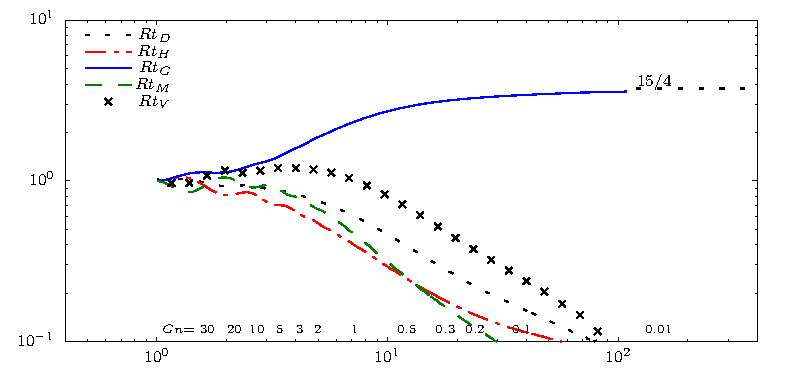
\includegraphics{ee}
\end{center}
 \caption{Plot of the five statistically independent contributions to
   $\epsilon$, normalised as in \eqref{epsRatios}, for Case II.
\label{fig:late-time-epsilon} }
\end{figure}
%%
Both of these conditions are observed in figure \ref{fig:late-time-epsilon},
which shows the ratios for case II.  At early times, each of the ratios is
approximately unity whereas at late time $Rt_G$ appears to by asymptoting
to 15/4.

The results from other studies exhibit this behaviour of the dissipation rate
as well.  Both \cite{fincham96} and \cite{praud05} performed experiments in
salt-stratified tanks, and both generated turbulence by towing a vertical grid
through the tank.  At the later stages of decay in both experiments the value
of $\Gn$ had dropped to values well below one.  In addition, the flows had
become approximately horizontal, and in both experiments it was reported that
the ratio $Rt_G$ was well above 0.9.  These features for both experiments all
indicate the approximate validity of \eqref{eqn:godoy} at later times.
\cite{hebert06b} performed direct numerical simulations in a strongly
stratified fluid of the decay of flows initially consisting of Taylor-Green
vortices, similar to the work of \cite{riley03}, but over a very broad range
of Reynolds number, Froude number, and $\Gn$.  They found that the ratio
$Rt_G$ is a very strong function of $\Gn$, and that $Rt_G$ being near 0.9 only
occurred when $Gn$ was order one or less.  From the present results, and from
these experimental and numerical results, there is reason to speculate that
\eqref{eqn:godoy} hold in many other flows that are strongly stratified and
$Gn$ is small.

%These equations describe the late-time behaviour of the present case, as well as that for a number of stably-stratified, laboratory flows which are dominated by lower Reynolds number, quasi-horizontal motions.  For example, \cite{fincham96}, in studies of the late wake of a grid towed in a salt-stratified tank, found that about 80\% of the dissipation rate was contributed by the terms containing the vertical gradient of the horizontal velocity.  It is possible that many flows in the quasi-two-dimensional regime with low Froude number and low Reynolds number are described by these equations.

%It is interesting to observe the behaviours of all three cases in the $\Fh$-$Gn$ plane, as %in figure~\ref{fig:gn}.  Note the change in the slope of all three curves at about $T=1$, %corresponding to the adjustments of the decay rates of $u$ and $v$ observed in %figure~\ref{fig:urms}.  As seen in the figure, this occurs when $\Fh$ has dropped to a %value of about 0.6.  We take this to be the value of $\Fh$ when a flow has entered the %strongly stratified regime, and decays at a rate approximately consistent with the %prediction of \citet{davidson10}.  Second, note from figure~\ref{fig:rho} for $\rho'$, %figure~\ref{fig:energy}(b) for energy, figure~\ref{fig:mixing_efficiency} for $\eta$, and %figure~\ref{fig:gn} for $\Rb$, that the low Reynolds number case, Case I, begins to %significantly deviate from the higher Reynolds number cases, Cases II and III, at about %$T=2$, corresponding to approximately $Gn = 0.5$.  We take this to be the value of $Gn$ %below which the flow does not remain turbulent.  We note from these criteria that Cases II %and III remain in the turbulent regime throughout the course of the simulations.
%%
%%
\afterpage{\clearpage}
\section{Conclusions and Discussion}

Direct numerical simulations were used to study the effects of stable ambient density stratification on initially isotropic turbulence.  To initialise the stratified flows, and for comparison with cases with stratification, first of all three non-stratified cases were run at three different Reynolds numbers.  It was found that all three flows attained approximately self-similar decay, with r.m.s.\ decay rates of approximately $t^{-0.56}$, and integral scale growth rates of approximately $t^{0.44}$.  These values are not far from the rates of $t^{-0.6}$ and $t^{0.4}$ predicted for Saffman turbulence \citep{saffman67}, and observed in some laboratory data.  Therefore, these non-stratified cases are useful for the initialisation of and comparison with the cases with stratification. 

In the cases with stable stratification, analogous to the results of \cite{spedding97}, as the flows decay we find that they traverse three different regimes which depend on the local Froude number, $\Fh$, and activity parameter, $\Gn$.  In the first regime, the weakly stratified regime, which occurs up to approximately one buoyancy period,  when $\Fh$ is above about 0.6, the flows follow their non-stratified counterparts.  By about one buoyancy period, however, the flows have adjusted to the stable stratification as the value of $F_h$ falls below 0.6.  If $Gn$ remains high enough, then the flows enter the second regime, which we term the stratified turbulence regime, and proceed to decay in a manner similar to that predicted by \cite{davidson10}, and to satisfy the scaling analysis of \cite{billant01}.  In particular, the horizontal r.m.s.\ velocity decay rates are reduced, the growth rates of the horizontal integral scales of the horizontal velocities increase, while the vertical integral scales of the horizontal velocities begin to decrease.  Finally, when the activity parameter decays to a value in the range of 0.1 to 1, the flows enter into the third regime, the viscous dominated regime.  Here the flow dynamics have changed considerable and follow the scaling analysis of \cite{godoy-diana04}.  In particular the vertical velocity becomes very small compared to the horizontal velocities, and the kinetic energy dissipation rate is dominated by the vertical shearing of the horizontal motions.

The results regarding the decrease in decay rate in the stratified turbulence regime are at least qualitatively consistent with the data from several laboratory experiments \citep{lin79,spedding97,yoon90, stillinger83}.  They are inconsistent, however, with the results of several other laboratory experiments \citep{liu95, praud05, itsweire86}.  It is not clear why our results differ from some of the experimental results, and why in fact some of the experimental results differ from one another while performed under seemingly similar conditions.  
As mentioned in the introduction, a key difference between our simulations and the laboratory experiments is how the flows are initialised.  Our flows have achieved close to a classical isotropic, homogeneous, decaying turbulent flow before the stratification is imposed.  On the other hand in the laboratory experiments the stratification exists before the turbulence is generated. Generally in the laboratory experiments where a grid of mesh size $M$ is used to generate the turbulence, a certain distance from the grid, say $x_0/M$, is required before the flow begins to decay in a self-similar manner.  Taking $U$ to be the speed of the grid relative to the fluid, and with $t_0 = x_0/U$ as the time it takes for the flow to become self-similar, then, in terms of buoyancy periods, this is $Nt_0/2 \pi = (x_0/M)(NM/2 \pi U) = (x_0/M)/Fr$.  In many of the laboratory experiments, $Fr \sim (x_0/M)$, suggesting that the flows are often modified by stratification before they begin self-similar decay.  These facts would suggest a change in decay behaviour different from what is obtained in our simulations; but it would not indicate how the decay rates would be different.

There are several interesting features of the flows in the stratified
turbulence regime.  For example, the vertical component of the kinetic energy
decays at a faster rate than the two horizontal components while, after its
initial adjustment, the density fluctuation $\rho'$ decays at approximately
the same rate as does $u_h$.  From an energetics perspective, this indicates
that the potential energy decays at approximately the same rate as the
horizontal components of the kinetic energy. This could be due to the density
field trying to stay in cyclostrophic adjustment with the horizontal
components of the velocity field.  Another feature of this regime is the
behaviour of the local Froude numbers; the Froude number $\Fh$ continues to
decay, while $Fr_v$ becomes approximately constant, consistent with the
predictions of \cite{billant01}.  Furthermore, in the stratified turbulence
regime, for the two higher Reynolds number cases, the mixing efficiency
asymptotes to approximately 0.35. This is roughly consistent with a number of
numerical simulations with $Pr = {\cal O}(1)$
\citep{smyth01,riley03,almalkie12a,maffioli16b}.  The lowest Reynolds number
case is only briefly in the stratified turbulence regime, however.  After
about 2 buoyancy periods its activity parameter has dropped well below 1 as it
enters the viscous-dominated regime; its mixing efficiency as well as $F_v$
begin to decay.
%This could be explained as the flow evolving into a system of internal waves that are coming into equipartition.  This is unlikely, however, as there is a significant amount of vertical vorticity, and hence potential vorticity, in the flow field, inconsistent with the assumption of field of internal waves.  Another explanation is that the flow consists of a field a quasi-horizontal vortices, and that the density field is in cyclostrophic adjustment with these vortices.  The final answer, however, might be a combination of these two and other explanations in combination.

%Another interesting feature of the flow is that the vertical component of the kinetic energy decays at a faster rate than the two horizontal components.  This could help to lead to the development of the quasi-horizontal vortices, or `pancake eddies', observed for later times in the experiments.  In the experiments for the wake of an isolated object, however, part of this bias is due to the loss of energy in the wake to internal wave radiation \citep{watanabe16}.  For short times in the simulations, this difference in energy components is partially explained by the fast gain in potential energy as the flow adjusts to the stable stratification. For later times, the vertical component continues to decay faster, however.  For these later times, it is possible that this bias is similar to the flow near the surface of a (relatively flat) river, which can be considered a very strongly stratified layer.  In this region the vertical velocity is suppressed as the flow approaches the river surface \citep{hunt78}.

%For the two higher Reynolds number cases, as the flows traverse the strongly stratified regime ($Fr < 1$), the mixing efficiency asymptotes to approximately 0.35.  This is roughly consistent with a number of numerical simulations with $Pr = {\cal O}(1)$ \citep{smyth01,riley03,almalkie12a,maffioli16b}.  For the lower Reynolds number case, however, when stratification effects become important, the mixing efficiency continues to decay with time.  This is consist with the fact that, in the lowest Reynolds number case, the activity parameter $Gn$ is ${\cal O}(1)$ when the flow enters the strongly stratified regime, indicating that it is no longer turbulent.  On the other hand, the two higher Reynolds number cases appear to remain turbulent for several buoyancy periods after the flows have entered the strongly stratified regime.

The horizontal spectra of the horizontal components of the velocity behave
very differently in the stratified cases compared to the non-stratified cases.
Initially the spectra for these flows have a moderate inertial range, with a
bump in the compensated spectra sometimes attributed to a ``bottleneck'' in
the energy transfer to smaller scales.  As each flow evolves into the
stratified turbulence regime, however, a peak in the compensated spectra
arises and continues to grow at about wave number $\kappa_x L_k =
8\cdot10^{-3}$.  In addition, in examining the horizontal spectra of various
shear terms, it is found that the spectra of $\partial u/\partial x$,
$\partial v/\partial y$, and $\partial w/\partial z$ evolve in a very similar
manner, again supporting the scaling arguments of \cite{billant01}. Even at
moderate times the vertical shearing of the horizontal component of the
velocity at somewhat low wave numbers begins to dominate, indicating that
vertical shear layers are probably driving the turbulence.

When $\Fh$ is below 0.6 and the value of $Gn$ drops below between 1 and 0.1,
the flows enter the third regime, the viscous-dominated regime.  Here the flow
dynamics change again.  Now the horizontal components of the velocity decay at
a faster rate, similar to the decay rate in the first regime.  In addition,
the vertical velocity and density fluctuations decay at a much faster rate, as
the flow becomes approximately horizontal.  In this viscous dominated regime,
the flow behaviour appears to be consistent with \eqref{eqn:godoy}, based upon
the scaling arguments of \cite{godoy-diana04}.

It should be mentioned that, as listed in Table~\ref{tbl:parameters}, a fourth
case was simulated, Case~IV, with the same initial Reynolds number as
Case~III, but with a different initial Froude number, in this case $\F_h=1$.
This would possibly allow the examination of the effect of the initial Froude
number, and would permit the flow to enter into the stratified turbulence
regime earlier in time and so more energetic.  Since the activity parameter is
proportional to $1/\hat N^2$, however, when the flow for Case~IV enters into
the stratified turbulence regime, its Froude number $\F_h$ and activity
parameter $Gn$ have almost identical values as for Case~III, so that the flow
behaviour was very similar to that of Case~III.  Therefore the results for
Case~IV are not presented.

%Finally, to summarise, analogous to the laboratory studies of \cite{spedding97}, we find that the flows pass through three different regimes, depending on the values of $\Fh$ and $\Gn$.  In the first regime, for values of $\Fh$ above about 0.6, and assuming $\Gn$ is large enough, the flows decay at almost the same rate as non-stratified flows.  In the second regime, which we term the strongly stratified regime, for values of $\Fh$ below about 0.6 but $\Gn$ larger than about 1, the decay rates of $u_h$ decrease, and growth rates of $L_{ux}$ increase, similar to the predictions of \citet{davidson10}.  Finally, in the third regime, when $\Gn$ has fallen below a value between 1 and 0.1, the decay rates of $u_h$ again increase while $\rho'$ and $w'$ decrease precipitously as the flows become quasi-two-dimensional.

%\begin{itemize}

%\item do we need this section?

%\item why are the simulated decay rates so different from those from some of the lab experiments?

%\item other issues to discuss?

%\end{itemize}

%%
%%
%\section{Conclusions}

%\begin{itemize}

%\item modification of the decay rates of kinetic energy, growth rates of integral scales, similar to the prediction of \cite{davidson10}

%\begin{itemize}

%\item qualitatively consistent with Spedding's \citep{spedding97} diagram

%\end{itemize}

%\item decay of $Fr$ approximately independent of $Re$. (figure 17 strongly supports this for $\Fh$)

%\item $E_h$ grows increasingly larger than $E_w+E_p$ and the flows decay.

%\item tendency towards stratified inertial range attained for $\Rb \ge 10$

%\begin{itemize}

%\item insufficient resolution to treat both stratified turbulence and Kolmogorov inertial ranges

%\end{itemize}

%\item mixing efficiency asymptotes to about 0.30 -- 0.35 for $\Rb \ge 10$

%\item able to achieve strongly stratified regime with ${\cal R} > 1$ for the two highest $Re$ cases.

%\item $\epsilon \sim u_{rms}^3/L_h$ 

%\item velocity gradient spectra consistent with \cite{bil01} scaling for continuity equation

%\item stable stratification enhances vertical shear, as suggested by \cite{lilly83}, \cite{bil01}

%\begin{itemize}

%\item consider this crucial to subsequent dynamicss

%\end{itemize}

%\end{itemize}
%%
%%

%%
%%

%%

%%

%\begin{figure}
%\begin{center}
% \includegraphics[width=5in]{l11}
%\caption{Averaged longitudinal integral lengths of horizontal velocities.}
%\end{center}
%\end{figure}

%\begin{figure}
%\begin{center}
 %\includegraphics{Plots/Spec2d/R160F2}
%\hspace*{-40pt}
 %\includegraphics{Plots/Spec2d/R2325F2}
%\end{center}
%\caption{Cylinder-averaged spectra of horizontal (solid lines) and vertical
%  (dashed lines) contributions to kinetic energy.  Curves are labeled
%  with $t \ (T)$.  The reference slopes are in the same location in both panels.}
%\end{figure}

%\begin{figure}
%\begin{center}
 %\includegraphics{R2325h}
%\hspace*{-20pt}
% \includegraphics{R2325v}
%\end{center}
%\caption{Horizontal and vertical one-dimensional spectra for case R2325F2.
%  Times are offset in increments of decades.  
%\label{fig:specv}}
%\end{figure}



%\begin{figure}
%\begin{center}
% \includegraphics[width=5in]{Plots/Ozmidov/longitudinal2325}
%\caption{Velocity longitudinal autospectra for case R2325F2.}
%\end{center}
%\end{figure}

%\begin{figure}
%\begin{center}
% \includegraphics[width=5in]{Plots/Ozmidov/transverse2325}
%\caption{Velocity transverse spectra in the $x$-direction for case
%  R2325F2. Horizontal velocity (black), vertical velocity (red).}
%\end{center}
%\end{figure}


%\begin{figure}
%\begin{center}
% \includegraphics[width=5in]{froude}
% \includegraphics[width=5in]{reynolds}
%\caption{Horizontal Froude, Reynolds and buoyancy Reynolds numbers.}
%\end{center}
%\end{figure}


%\begin{figure}
%\begin{center}
% \includegraphics[width=5in]{Fmaffioli}
%\caption{Mixing efficiency $\Gamma=\chi/\epsilon$.  Late times are to the left.}
%\end{center}
%\end{figure}

%\subsection{Shear Spectra}

%\begin{figure}
%\begin{center}
 %\includegraphics{khspec}
%\caption{Two-dimensional spectra of vertical derivative of horizontal
%  velocity.  Colors indicate log10 of shear energy.  Case R2325F2.}
%\label{fig:khspec}
%\end{center}
%\end{figure}

%\begin{figure}
%\begin{center}
 %\includegraphics{kxspec}
%\caption{One-dimensinal spectra of various shear terms versus $\kappa_x$. Case R2325F2.}
%\label{fig:kxspec}
%\end{center}
%\end{figure}

%\begin{figure}
%\begin{center}
% \includegraphics{kzspec}
%\caption{One-dimensinal spectra of various shear terms versus $\kappa_z$.
%  Case R2325F2. See
%figure \ref{fig:kxspec} for legend. }
%\label{fig:kzspec}
%\end{center}
%\end{figure}

%\begin{acknowledgments}
\section*{Acknowledgements}
This work was funded by the Office of Naval Research via grant
N00014-12-1-0583.  High performance computing resources were provided through
the U.S.\ Department of Defense High Performance Computing Modernization
Program by the Army Engineer Research and Development Center and the Army
Research Laboratory under Frontier Project FP-CFD-FY14-007.
%\end{acknowledgments}

\bibliographystyle{jfm}
\bibliography{bib}

%%
%%
\end{document}


%<!-- Local IspellDict: en_GB  -->
